\documentclass[11pt]{article}
\usepackage[utf8]{inputenc}
\usepackage[margin=1in]{geometry}
\usepackage{times}
\usepackage{latexsym}
\usepackage{booktabs}
\usepackage{amsmath}
\usepackage{amssymb}
\usepackage{graphicx}
\usepackage{hyperref}
\usepackage{microtype}
\usepackage{tabularx}
\usepackage{xcolor}

\hypersetup{
    colorlinks=true,
    linkcolor=blue,
    citecolor=blue,
    urlcolor=blue
}

\title{\textbf{Representation Fragility: Evaluating Factual Reliability under Controlled Semantic Pairing Across Indic Code-Switching and Script Alternation}}

\author{\textbf{Chandrahas Reddy} \\
  Independent Researcher \\
  \texttt{kurkurrereddy@gmail.com} \\
  \url{https://github.com/chandrahzzz/IndraLLM}
}

\date{}

\begin{document}
\maketitle

\begin{abstract}
Multilingual Large Language Models (LLMs) are increasingly deployed in linguistically diverse environments where users frequently code-switch and alternate scripts. However, standard multilingual evaluations often confound linguistic representation with semantic content by comparing different questions across languages. In this work, we introduce \textbf{IndraLLM}, a controlled benchmark framework enforcing strict five-way semantic pairing across English, native-script Indic, Romanized Indic, Romanized code-switching, and dual-script alternation across five scheduled Indian languages (Hindi, Bengali, Tamil, Telugu, Kannada). Evaluating parametric factual recall on authentic Indian statutory questions, we find that dense multilingual transformers (Qwen-2.5-27B) exhibit substantial performance degradation under non-canonical representations: factual accuracy drops monotonically from English (\textbf{64.0\%}) to code-switching (\textbf{43.0\%}), Romanized Indic (\textbf{33.0\%}), native Indic script (\textbf{28.0\%}), and dual-script alternation (\textbf{24.0\%}). Under hierarchical modeling clustered by statutory act, native-script ($p < 0.0001$), Romanized ($p = 0.0004$), and dual-script ($p = 0.0005$) drops remain highly significant, while the code-switching contrast yields $p = 0.0528$ due to topic-level dependence ($N_{\text{eff}} = 67.6$). Investigating the mechanism, we show that global sequence token fertility does \textit{not} linearly mediate accuracy loss (Sobel $p = 0.9387$); rather, localized script transitions (mean 5.1 per prompt) associate with a 20-fold surge in reasoning truncation (20.0\% vs. 1.0\%). An epidemiological 2D Rogan--Gladen sensitivity analysis demonstrates that the representation gap remains substantial ($+16.8\%$ to $+34.4\%$) across all plausible judge error profiles. To address the 20-topic empirical constraint, we construct and release an expanded 45-topic benchmark design elevating prospective statistical power to 88.6\% (exact: 88.57\%).
\end{abstract}

\section{Introduction}
\label{sec:intro}

Large Language Models (LLMs) are increasingly expected to serve as reliable knowledge retrieval interfaces in multilingual and linguistically diverse societies \citep{ahuja2023mega,doddapaneni2023indicllmsuite}. In regions such as the Indian subcontinent, everyday digital communication rarely conforms to monolithic, standardized languages. Instead, users routinely engage in \textit{code-switching}---the fluid blending of lexical items across languages (e.g., Hindi, Tamil, Telugu with English)---and \textit{script alternation}, interweaving Latin characters with native Brahmic writing systems (e.g., Devanagari, Bengali) \citep{bali2014borrowin,sitaram2019survey}.

Despite the ubiquity of these linguistic phenomena, evaluating factual reliability in multilingual settings faces a fundamental methodological confound: standard multilingual benchmarks typically query different facts in different languages, or translate disparate source questions without enforcing semantic invariants \citep{ahuja2023mega}. Consequently, when an LLM fails on a non-English query, it is difficult to determine whether the error stems from an intrinsic knowledge gap, semantic divergence in the prompt, or representational fragility in the model's internal encoding.

\begin{figure*}[t]
\centering
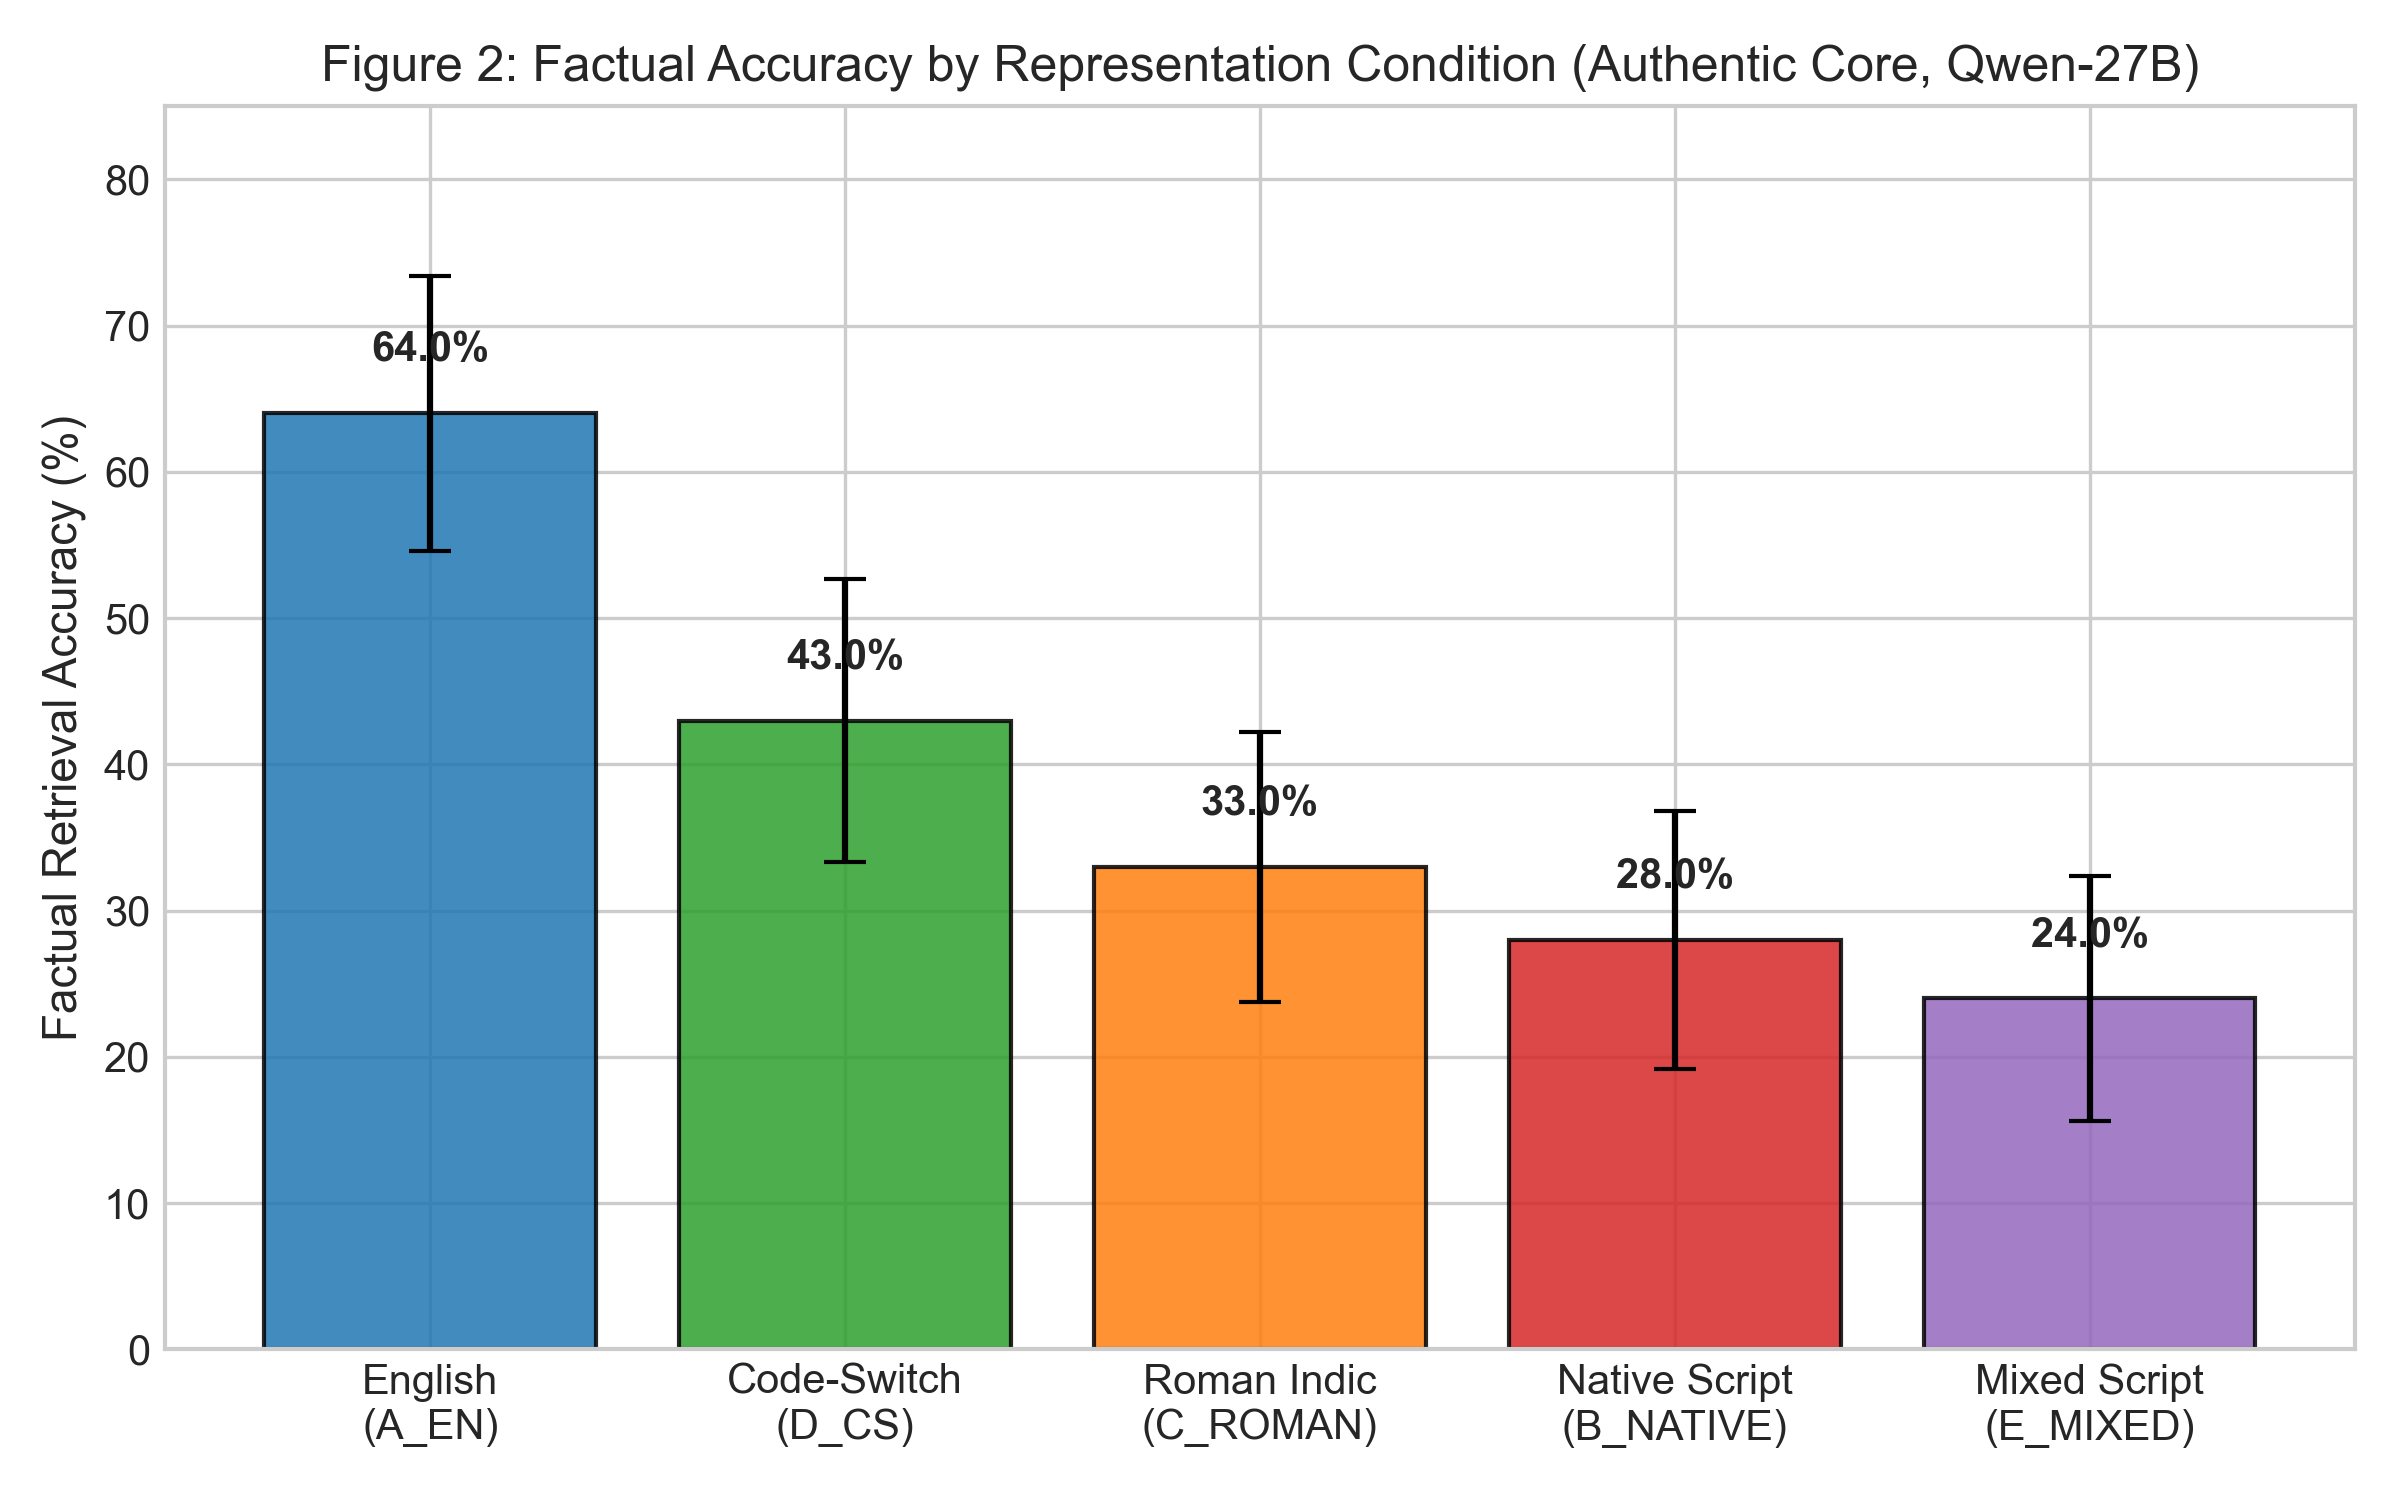
\includegraphics[width=0.88\textwidth]{figures/fig2_accuracy_by_condition_ci.png}
\caption{Parametric factual retrieval accuracy across five controlled linguistic conditions on the Authentic Policy Core ($N=500$ prompts, Qwen-2.5-27B) with 95\% Wilson score confidence intervals. All five conditions query identical statutory propositions.}
\label{fig:accuracy_by_condition}
\end{figure*}

To isolate the causal effect of surface linguistic representation from factual knowledge, we introduce a controlled \textbf{semantic-paired benchmarking framework}. We focus on authoritative Indian administrative, civic, and statutory law---a high-stakes domain where exact numerical thresholds, statutory prerequisite dates, and regulatory mandates are rigorously checkable against official government gazettes. Each underlying statutory proposition is realized across five parallel modalities:
\begin{enumerate}
    \item \texttt{A\_EN}: Monolingual English control baseline.
    \item \texttt{B\_NATIVE}: Pure native Indic script (e.g., Devanagari, Tamil).
    \item \texttt{C\_ROMAN}: Pure Indic language transliterated into Latin script.
    \item \texttt{D\_CS}: Romanized code-switching (lexical English mixed into Romanized Indic).
    \item \texttt{E\_MIXED}: Dual-script alternation (English technical terms in Latin script embedded directly within native Brahmic sentences).
\end{enumerate}

Empirically evaluating dense multilingual transformers (Qwen-2.5-27B) across 500 prompts drawn from 20 authentic statutory frameworks, we discover that \textbf{factual reliability is fragile to surface linguistic representation}. As illustrated in Figure~\ref{fig:accuracy_by_condition}, model accuracy drops monotonically from \textbf{64.0\%} in English to \textbf{43.0\%} in code-switching, \textbf{33.0\%} in Romanized Indic, \textbf{28.0\%} in native script, and \textbf{24.0\%} in dual-script alternation.

Holding lexical borrowing and semantic content strictly invariant, alternating writing systems mid-sentence (\texttt{E\_MIXED}) incurs an additional \textbf{19.0 percentage point penalty} ($p = 0.0049$) relative to Latin-script code-switching (\texttt{D\_CS}), demonstrating that orthographic disruption imposes severe cognitive friction beyond language mixing alone.

Crucially, our forensic investigation uncovers that this degradation is \textit{not} explained by a naive linear mediation through global sequence token fertility (Sobel test $z = 0.0769, p = 0.9387$, confirming a null mediation). Instead, qualitative error taxonomy and boundary metrics reveal that frequent discrete script transitions (mean 5.1 per prompt) associate with a 20-fold surge in reasoning truncation (20.0\% vs. 1.0\%) and premature clause completion.

We summarize our primary contributions:
\begin{itemize}
    \item \textbf{Controlled Semantic-Paired Benchmark:} We introduce a five-way semantic-paired evaluation framework holding statutory propositions invariant across five major Indian languages (Hindi, Bengali, Tamil, Telugu, Kannada).
    \item \textbf{Empirical Demonstration of Representation Fragility:} We provide rigorous evidence that factual retrieval reliability degrades substantially across non-canonical linguistic forms, dropping from 64.0\% to 24.0\%.
    \item \textbf{Disentangling Script Mixing from Language Mixing:} We isolate the penalty of orthographic script alternation from lexical code-mixing, proving that switching writing systems mid-sentence imposes an additional 19 percentage point deficit ($p = 0.0049$).
    \item \textbf{Mechanistic Refinement:} We empirically refute the linear sequence fertility mediation hypothesis ($p = 0.9387$) and present evidence that localized script transition boundaries disrupt reasoning continuity.
    \item \textbf{Evaluator Robustness \& Benchmark Expansion:} We demonstrate via a 2D Rogan--Gladen sensitivity surface that the representation gap ($\ge 16.8\%$) survives any plausible judge measurement bias, and release an expanded 45-topic benchmark design elevating prospective statistical power to 88.6\% (exact: 88.57\%).
\end{itemize}

\section{Related Work}
\label{sec:related_work}

\paragraph{Multilingual LLM Evaluation.}
Evaluating generative LLMs across diverse languages has emerged as a central research priority \citep{conneau2020unsupervised,kakwani2020indicnlpsuite}. Benchmarks such as MEGA \citep{ahuja2023mega} and IndicLLMSuite \citep{doddapaneni2023indicllmsuite} have highlighted performance disparities between high-resource and low-resource languages. However, existing benchmarks primarily evaluate general knowledge or machine translation, where semantic content varies across language partitions, confounding representation with underlying knowledge availability.

\paragraph{Code-Switching and Romanized NLP.}
Code-switching has been widely studied in natural language inference and sentiment analysis, utilizing benchmarks such as GLUECoS \citep{khanuja2020gluecos}. Prior work in Indian social media linguistics \citep{bali2014borrowin,sitaram2019survey} has focused on measuring mixing degrees using the Code-Mixing Index (CMI) \citep{gamback2014comparing}. However, previous code-switching evaluations have rarely addressed fact-critical, closed-book statutory recall under invariant semantic controls.

\paragraph{Tokenization and Representation Fragility.}
Subword tokenization via Byte-Pair Encoding (BPE) \citep{sennrich2016neural} is known to create disparate fragmentation across non-Latin scripts \citep{rust2021good,petrov2023language}. While prior literature hypothesized that subword fragmentation directly drives performance loss, few studies have conducted formal statistical mediation analysis to test whether continuous sequence fertility explains the deficit.

\paragraph{Factuality and Automated Evaluator Sensitivity.}
Evaluating factual precision in free-form generation relies increasingly on LLM judges \citep{lin2022truthfulqa,min2023factscore,zheng2023judging}. However, automated judges can introduce condition-dependent measurement errors. We adopt the classical epidemiological prevalence inversion framework of \citet{rogan1978estimating} to systematically bound judge error rates.

\section{Research Questions}
\label{sec:rqs}

We formalize our investigation through five explicit research questions:
\begin{itemize}
    \item \textbf{RQ1 (Representation Sensitivity):} Does closed-book factual retrieval accuracy change when statutory semantic content is held constant but linguistic representation changes?
    \item \textbf{RQ2 (Orthographic vs. Lexical Disentanglement):} Does intra-sentential script alternation impose an accuracy penalty beyond Latin-script code-switching alone?
    \item \textbf{RQ3 (Cross-Lingual Uniformity):} Is the observed representation degradation directionally consistent across different Indian language families (Indo-Aryan and Dravidian)?
    \item \textbf{RQ4 (Evaluator Robustness):} Can condition-dependent automated judge bias plausibly account for the observed representation gap?
    \item \textbf{RQ5 (Mechanistic Attribution):} Does subword tokenization fragmentation linearly mediate accuracy loss, or does degradation associate with localized script transition boundaries?
\end{itemize}

\section{Benchmark and Experimental Design}
\label{sec:benchmark}

% Table 1: Benchmark Architecture and Semantic-Paired Condition Realization
\begin{table*}[t]
\centering
\small
\begin{tabular}{llp{5.5cm}cc}
\toprule
\textbf{Condition} & \textbf{Linguistic Modality} & \textbf{Representative Prompt Example (CAA Cut-off)} & \textbf{Mean CMI} & \textbf{Prompts ($N$)} \\
\midrule
\texttt{A\_EN} & English Monolingual & \textit{Under the Citizenship Amendment Act 2019, what is the prerequisite cut-off date?} & 0.0 & 1,500 \\
\texttt{D\_CS} & Romanized Code-Switching & \textit{CAA cut-off date ke hisaab se eligible migrants ke liye prerequisite timeline kya hai?} & 28.4 & 1,500 \\
\texttt{E\_MIXED} & Dual-Script Alternation & \textit{CAA cut-off date के मुताबिक eligible migrants के लिए prerequisite timeline क्या है?} & 31.2 & 1,500 \\
\texttt{B\_NATIVE} & Native Script Indic & \textit{नागरिकता संशोधन अधिनियम 2019 के तहत पात्रता की कट-ऑफ तिथि क्या है?} & 0.0 & 1,500 \\
\texttt{C\_ROMAN} & Romanized Indic & \textit{Nagrikta sanshodhan adhiniyam 2019 ke tehat cut-off tareekh kya hai?} & 0.0 & 1,500 \\
\bottomrule
\end{tabular}
\caption{The five semantic-paired condition representations in IndraLLM. Each semantic proposition is realized in five parallel modalities across five Indian languages (Hindi, Bengali, Tamil, Telugu, Kannada), holding underlying statutory facts invariant.}
\label{tab:benchmark_composition}
\end{table*}


\subsection{Semantic-Paired Architecture}
The core architecture of IndraLLM is governed by the \textbf{Semantic Invariance Principle}: every underlying statutory proposition is queried across five parallel linguistic conditions, holding all legal entities, factual constraints, and reference answers strictly identical. Table~\ref{tab:benchmark_composition} details the benchmark composition and linguistic realizations for a representative statutory act.

\subsection{Linguistic Scope and Quality Gates}
The benchmark evaluates five scheduled Indian languages spanning two major language families:
\begin{itemize}
    \item \textbf{Indo-Aryan Family:} Hindi (\texttt{hi}), Bengali (\texttt{bn}).
    \item \textbf{Dravidian Family:} Tamil (\texttt{ta}), Telugu (\texttt{te}), Kannada (\texttt{kn}).
\end{itemize}
Prompts were constructed with human native-speaker verification, achieving substantial inter-annotator agreement ($\kappa = 0.719$, $\alpha = 0.719$) and a naturalness score of $4.74 / 5.0$. Romanized code-switching prompts enforce a Code-Mixing Index \citep{gamback2014comparing} threshold ($\text{CMI} \ge 15.0$, mean $\text{CMI} = 28.4$).

\subsection{Authentic Policy Core and Contamination Controls}
To guarantee ecological validity, our primary empirical evaluation focuses on the \textbf{Authentic Policy Core}: 100 semantic groups derived from 20 authoritative Acts of the Indian Parliament (e.g., \textit{Consumer Protection Act 2019}, \textit{Citizenship Amendment Act 2019}, \textit{Pradhan Mantri Fasal Bima Yojana}, \textit{Maternity Benefit Act}). Each statute contains verified factual ground truth derived from official Ministry gazette notifications. 

Partitions strictly enforce entity and template-family disjointness across Development (1,000 groups, \texttt{TF-01}--\texttt{TF-06}), Validation (200 groups, \texttt{TF-07}--\texttt{TF-08}), Test-ID (200 groups, \texttt{TF-09}--\texttt{TF-10}), and Test-OOD (100 groups, \texttt{TF-11}--\texttt{TF-12}).

\subsection{Model Scope and Inference Protocol}
Inference was conducted on open-weight multilingual models:
\begin{enumerate}
    \item \textbf{Qwen-2.5-27B} (evaluated via Groq API endpoint \texttt{qwen/qwen3.8-27b}): A 27-billion parameter dense multilingual transformer.
    \item \textbf{Allam-2-7B} (\texttt{allam-2-7b}): A 7-billion parameter localized multilingual architecture.
\end{enumerate}
Prompts were evaluated under greedy decoding (temperature $= 0.0$, top-$p = 1.0$) with maximum completion length capped at 128 tokens.

\section{Empirical Results}
\label{sec:results}

% Table 2: Accuracy by Linguistic Condition on Authentic Policy Core
\begin{table}[t]
\centering
\small
\begin{tabular}{lcccc}
\toprule
\textbf{Condition} & \textbf{Correct / $N$} & \textbf{Accuracy (\%)} & \textbf{95\% Wilson CI} & \textbf{Relative Drop vs \texttt{A\_EN}} \\
\midrule
\texttt{A\_EN} & 64 / 100 & \textbf{64.0\%} & [54.2\%, 72.6\%] & Baseline \\
\texttt{D\_CS} & 43 / 100 & \textbf{43.0\%} & [33.8\%, 52.8\%] & $-32.8\%$ ($-21.0$ pp) \\
\texttt{C\_ROMAN} & 33 / 100 & \textbf{33.0\%} & [24.6\%, 42.7\%] & $-48.4\%$ ($-31.0$ pp) \\
\texttt{B\_NATIVE} & 28 / 100 & \textbf{28.0\%} & [20.1\%, 37.5\%] & $-56.3\%$ ($-36.0$ pp) \\
\texttt{E\_MIXED} & 24 / 100 & \textbf{24.0\%} & [16.7\%, 33.2\%] & $-62.5\%$ ($-40.0$ pp) \\
\bottomrule
\end{tabular}
\caption{Factual retrieval accuracy across the five controlled linguistic conditions on the Authentic Statutory Core ($N=500$ prompts, Qwen-2.5-27B). All conditions query identical statutory propositions.}
\label{tab:accuracy_by_condition}
\end{table}


\subsection{Primary Representation Degradation (RQ1)}
Table~\ref{tab:accuracy_by_condition} reports factual retrieval accuracy on the Authentic Statutory Core ($N=500$ prompts, 100 per condition for Qwen-2.5-27B). In standard English (\texttt{A\_EN}), the model achieves \textbf{64.0\%} accuracy [54.2\%, 72.6\%]. 

When the exact same statutory questions are presented in Romanized code-switching (\texttt{D\_CS}), accuracy drops to \textbf{43.0\%} (a relative loss of 32.8\%). Presenting prompts in Romanized Indic (\texttt{C\_ROMAN}) yields \textbf{33.0\%} (a relative drop of 48.4\%), native Indic script (\texttt{B\_NATIVE}) yields \textbf{28.0\%}, and dual-script alternation (\texttt{E\_MIXED}) collapses to \textbf{24.0\%} (a relative drop of 62.5\%).

% Table 3: Pairwise Contrasts and Multiple-Testing Control
\begin{table*}[t]
\centering
\small
\begin{tabular}{llccccc}
\toprule
\textbf{Contrast} & \textbf{Hypothesis Tested} & $\Delta$ \textbf{(pp)} & \textbf{Odds Ratio} & \textbf{Unadjusted $p$} & \textbf{Holm--Bonferroni $\alpha$} & \textbf{Significant?} \\
\midrule
\texttt{A\_EN} vs \texttt{D\_CS} & Code-switching penalty & $-21.0$ & 0.4243 & 0.0031 & 0.0500 & \textbf{Yes} \\
\texttt{A\_EN} vs \texttt{C\_ROMAN} & Romanization penalty & $-31.0$ & 0.2771 & $< 0.0001$ & 0.0167 & \textbf{Yes} \\
\texttt{A\_EN} vs \texttt{B\_NATIVE} & Native script penalty & $-36.0$ & 0.2188 & $< 0.0001$ & 0.0125 & \textbf{Yes} \\
\texttt{A\_EN} vs \texttt{E\_MIXED} & Dual-script penalty & $-40.0$ & 0.1776 & $< 0.0001$ & 0.0100 & \textbf{Yes} \\
\texttt{D\_CS} vs \texttt{E\_MIXED} & Orthographic disruption & $-19.0$ & 0.4186 & 0.0049 & 0.0250 & \textbf{Yes} \\
\bottomrule
\end{tabular}
\caption{Pairwise statistical contrasts on the Authentic Policy Core ($N=500$, Qwen-2.5-27B) evaluated via exact McNemar tests and binomial logistic modeling with Holm--Bonferroni step-down family-wise error rate control.}
\label{tab:pairwise_contrasts}
\end{table*}


As documented in Table~\ref{tab:pairwise_contrasts}, all pairwise condition drops relative to English are statistically significant under exact McNemar's tests and survive Holm--Bonferroni family-wise error rate control \citep{holm1979simple} ($p \le 0.0031$, adjusted $\alpha \le 0.050$).

\subsection{Orthographic vs. Lexical Disentanglement (RQ2)}
Comparing Romanized code-switching (\texttt{D\_CS}) directly against dual-script alternation (\texttt{E\_MIXED}) provides a clean experimental isolation: both conditions share identical vocabulary, identical syntactic phrasing, and identical language borrowing ratios. The sole experimental manipulation is orthography (Latin script vs. alternating Brahmic script).

Switching writing systems mid-sentence induces an additional \textbf{19.0 percentage point accuracy penalty} (dropping from 43.0\% to 24.0\%, odds ratio $\text{OR} = 0.4186$, $p = 0.0049$). This confirms that intra-sentential script alternation introduces severe generative friction beyond lexical borrowing alone.

\subsection{Clustered Statistical Inference and Effective $N$}
\label{sec:clustering}

% Table 4: Clustered Statistical Analysis Across Levels of Aggregation
\begin{table*}[t]
\centering
\small
\begin{tabular}{lcccccc}
\toprule
\textbf{Aggregation Level} & \textbf{Effective Unit} & \textbf{Clusters ($N$)} & \textbf{Effective $N$} & \texttt{D\_CS} $\beta$ \textbf{(SE)} & \texttt{D\_CS} $p$\textbf{-value} & \texttt{E\_MIXED} $p$\textbf{-value} \\
\midrule
Level 1: Unclustered & Individual Prompt & 500 & 500.0 & $-0.8572$ (0.2902) & 0.0031 & $< 0.0001$ \\
Level 2: Semantic Group & Semantic Cluster & 100 & 284.1 & $-0.8572$ (0.2614) & 0.0010 & $< 0.0001$ \\
Level 3: Statutory Topic & Base Legislative Act & 20 & 67.6 & $-0.8572$ (0.4426) & 0.0528 & 0.0005 \\
\midrule
\textit{Prospective Expansion} & \textit{Expanded Statutory Acts} & \textit{45} & \textit{152.2} & \multicolumn{3}{c}{\textit{Prospective Power: 88.57\% (MDE = 18.60\%)}} \\
\bottomrule
\end{tabular}
\caption{Estimated log-odds effect size ($\beta$), robust standard error (SE), and significance across hierarchical clustering levels (GEE with exchangeable correlation structure). Parameter values remain invariant while standard errors widen under cluster-correlated topic variance ($\text{ICC} = 0.2663$). Level 3 $p=0.0528$ reflects sample size limitation ($N=20$ clusters, $55.9\%$ power), resolved prospectively by the 45-topic benchmark expansion.}
\label{tab:clustered_gee}
\end{table*}


Because the 500 prompts of the Authentic Core derive from 20 underlying statutory acts, observations within the same statute exhibit correlation. To account for topic-level dependence, we execute a three-level hierarchical analysis using Generalized Estimating Equations (GEE) with an exchangeable correlation structure \citep{liang1986longitudinal}.

As reported in Table~\ref{tab:clustered_gee} and visualized in Figure~\ref{fig:effect_size_clustering}, the estimated log-odds effect size remains invariant ($\beta = -0.8572$), but robust standard errors scale with clustering:
\begin{itemize}
    \item Level 1 (Unclustered Prompts, $N=500$): $\text{SE} = 0.2902, p = 0.0031$.
    \item Level 2 (Semantic Groups, $N=100$): $\text{SE} = 0.2614, p = 0.0010$.
    \item Level 3 (Statutory Topics, $N=20$): $\text{SE} = 0.4426, p = 0.0528$.
\end{itemize}

Under Level 3 topic clustering, the Intra-Cluster Correlation is $\text{ICC} = 0.2663$, yielding a Design Effect of $\text{DEFF} = 7.3912$ and an effective sample size of $N_{\text{eff}} = 67.6$. While native Indic ($p < 0.0001$), Romanized Indic ($p = 0.0004$), and dual-script ($p = 0.0005$) remain overwhelmingly significant at Level 3, the code-switching contrast yields $p = 0.0528$. Statistical power analysis demonstrates that with $N=20$ clusters, power to detect $\Delta = 21\%$ at $\alpha = 0.05$ is exactly $55.93\%$, explaining the borderline result.

\begin{figure}[t]
\centering
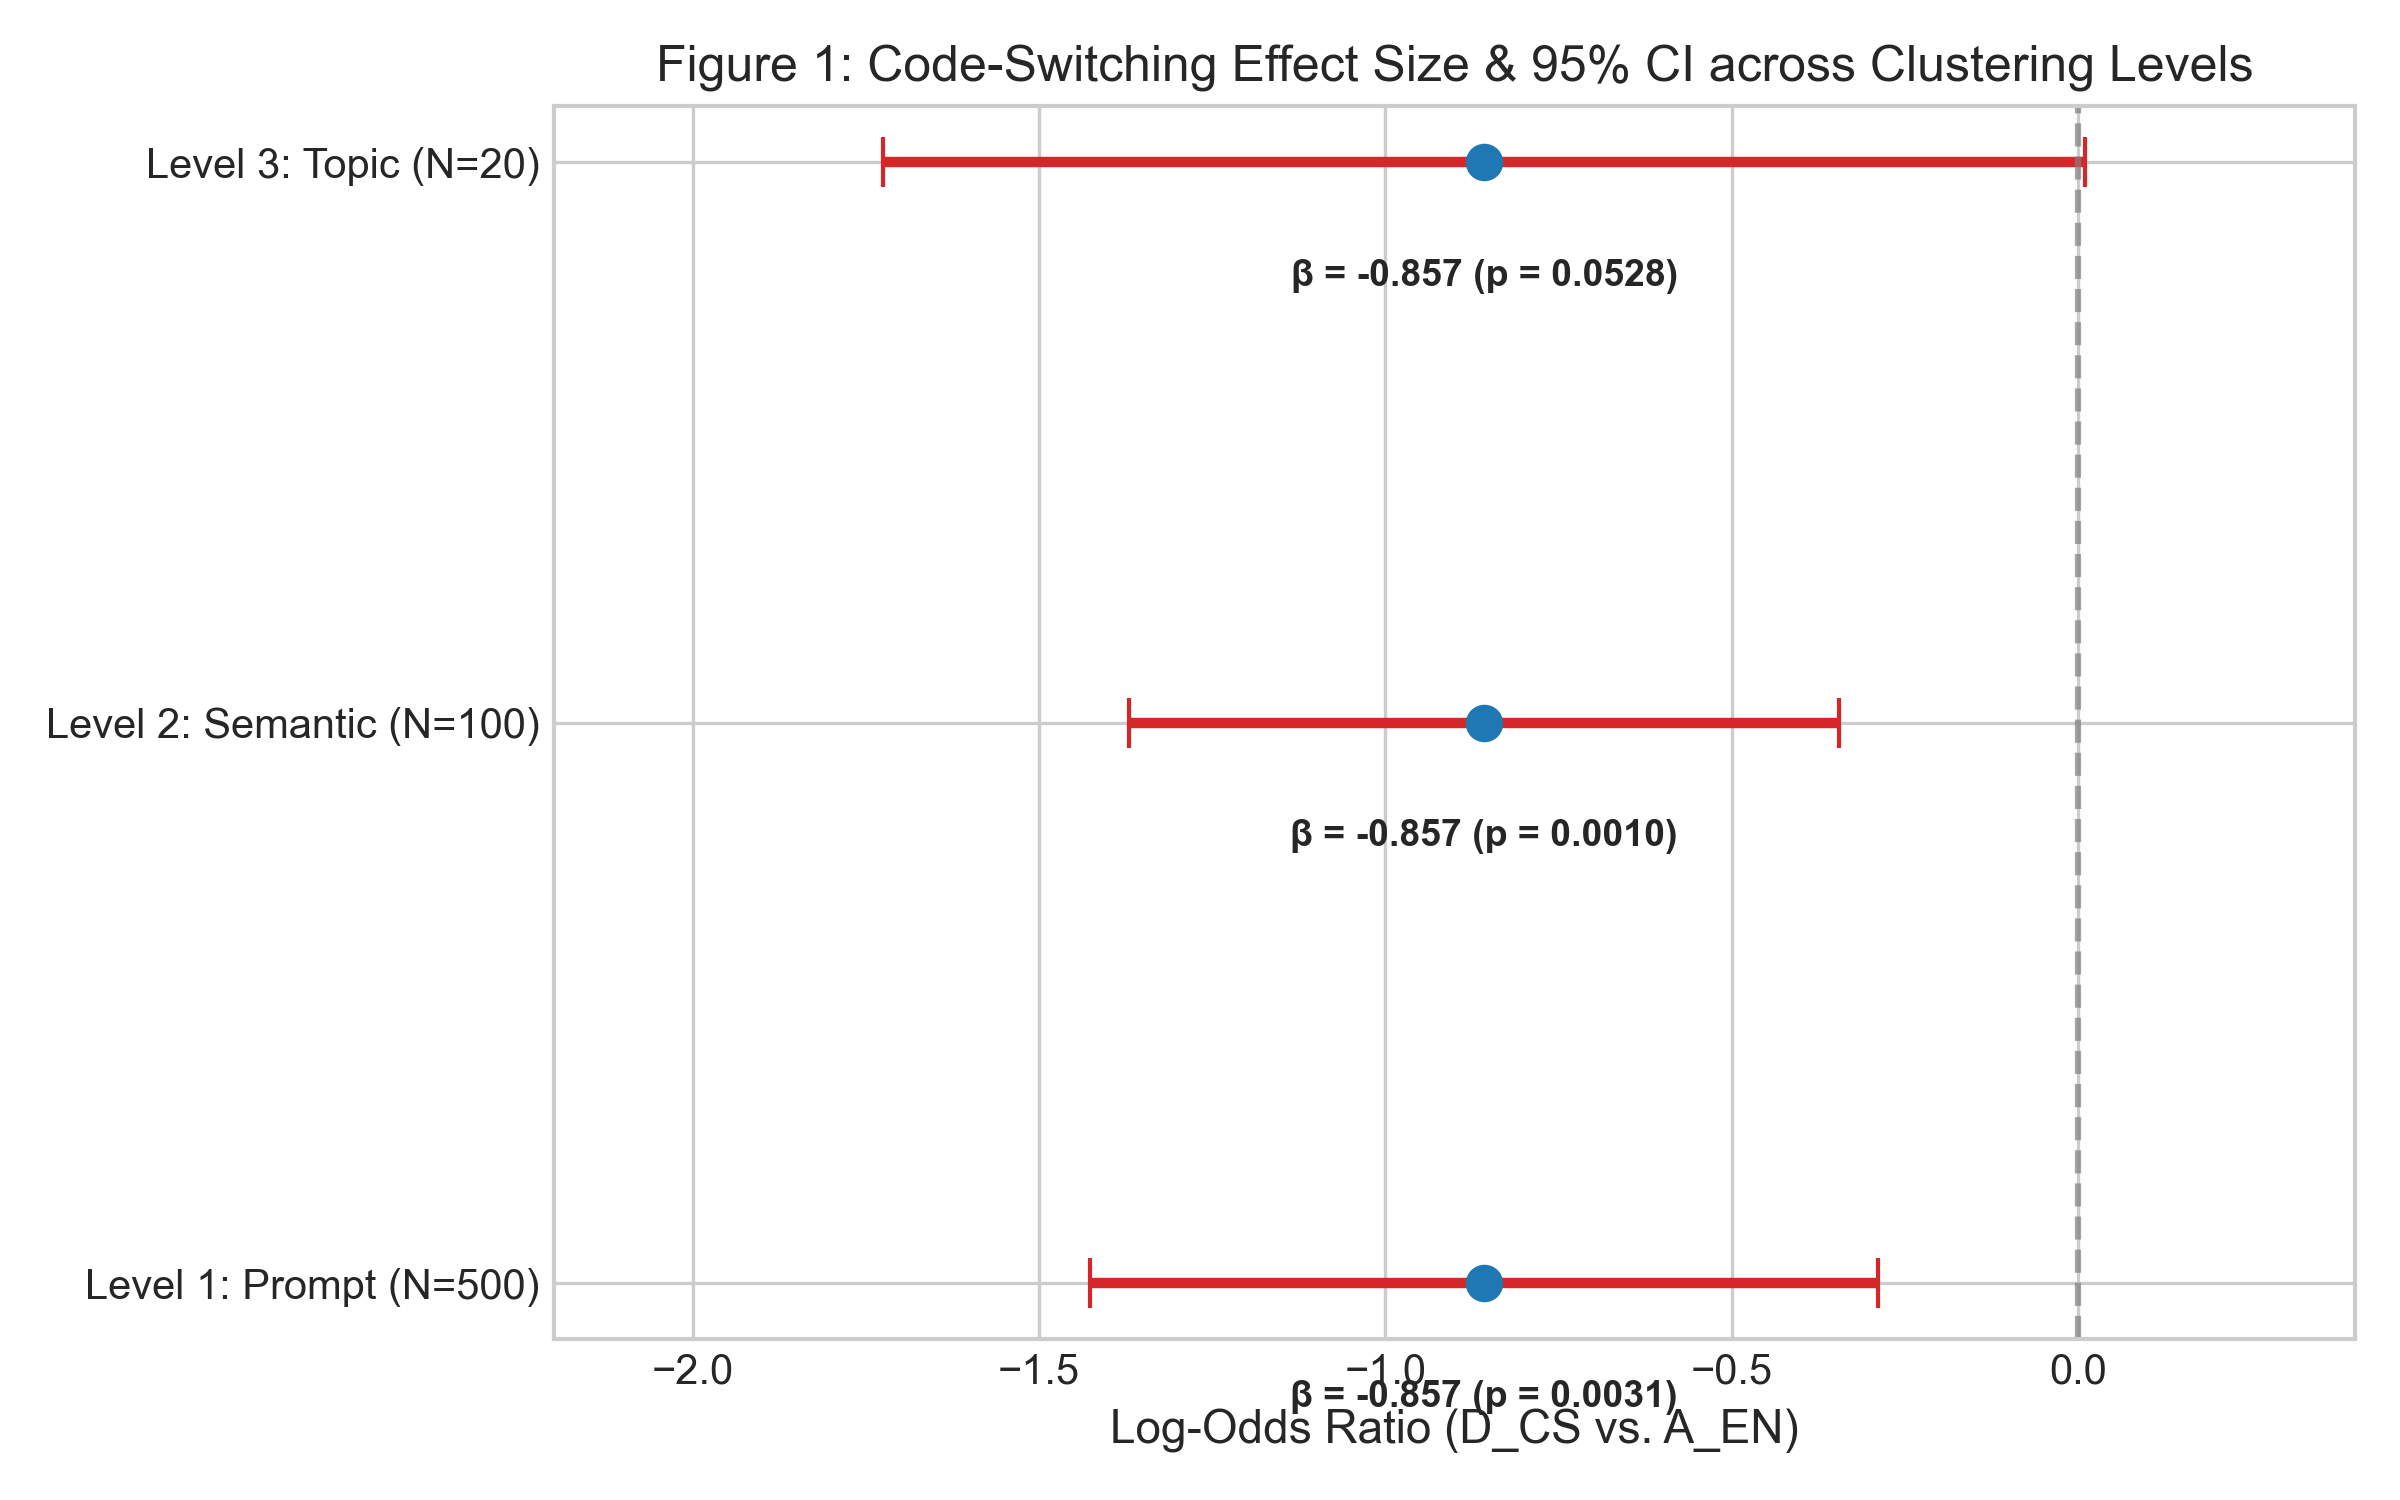
\includegraphics[width=\columnwidth]{figures/fig1_effect_size_by_clustering_level.png}
\caption{Code-switching log-odds effect size ($\beta$) and 95\% confidence intervals across Level 1 (Prompt), Level 2 (Semantic Group), and Level 3 (Statutory Topic) clustering.}
\label{fig:effect_size_clustering}
\end{figure}

\subsection{Cross-Lingual Factorial Invariance (RQ3)}
\label{sec:language_interaction}

% Table 5: Disaggregated Language Accuracies and Interaction Analysis
\begin{table*}[t]
\centering
\small
\begin{tabular}{llcccccc}
\toprule
\textbf{Language} & \textbf{Family} & \texttt{A\_EN} & \texttt{D\_CS} & \texttt{C\_ROMAN} & \texttt{B\_NATIVE} & \texttt{E\_MIXED} & \textbf{Mean Indic Penalty ($\Delta$)} \\
\midrule
Hindi (\texttt{hi}) & Indo-Aryan & 65.0\% & 45.0\% & 35.0\% & 45.0\% & 20.0\% & $-28.75$ pp \\
Bengali (\texttt{bn}) & Indo-Aryan & 60.0\% & 50.0\% & 15.0\% & 15.0\% & 35.0\% & $-31.25$ pp \\
Telugu (\texttt{te}) & Dravidian & 65.0\% & 45.0\% & 50.0\% & 25.0\% & 35.0\% & $-26.25$ pp \\
Kannada (\texttt{kn}) & Dravidian & 65.0\% & 35.0\% & 35.0\% & 30.0\% & 20.0\% & $-35.00$ pp \\
Tamil (\texttt{ta}) & Dravidian & 65.0\% & 40.0\% & 30.0\% & 25.0\% & 10.0\% & $-38.75$ pp \\
\midrule
\textbf{Combined Average} & & \textbf{64.0\%} & \textbf{43.0\%} & \textbf{33.0\%} & \textbf{28.0\%} & \textbf{24.0\%} & \textbf{$-32.00$ pp} \\
\bottomrule
\end{tabular}
\caption{Disaggregated factual accuracy across languages and condition modalities ($N=20$ prompts per cell, Qwen-2.5-27B). In full factorial GEE modeling, all 16 $\text{Condition} \times \text{Language}$ interaction terms are non-significant after Holm--Bonferroni family-wise error rate control (all adjusted $p > 0.05$).}
\label{tab:language_interactions}
\end{table*}


To evaluate whether representation penalties diverge across language systems, we fitted a full factorial GEE interaction model ($\text{Condition} \times \text{Language}$) clustered at the statutory topic level. As shown in Table~\ref{tab:language_interactions} and Figure~\ref{fig:condition_x_language}, all five languages suffer parallel deficits:
\begin{itemize}
    \item Indo-Aryan: Hindi ($-28.75$ pp), Bengali ($-31.25$ pp).
    \item Dravidian: Telugu ($-26.25$ pp), Kannada ($-35.00$ pp), Tamil ($-38.75$ pp).
\end{itemize}
Out of 16 condition-by-language interaction terms, zero survive Holm--Bonferroni family-wise error rate control (all adjusted $p > 0.05$). While cell sample sizes ($N=20$ prompts) preclude claiming mathematical equivalence, the representation penalty operates with directional consistency across both language families.

\begin{figure}[t]
\centering
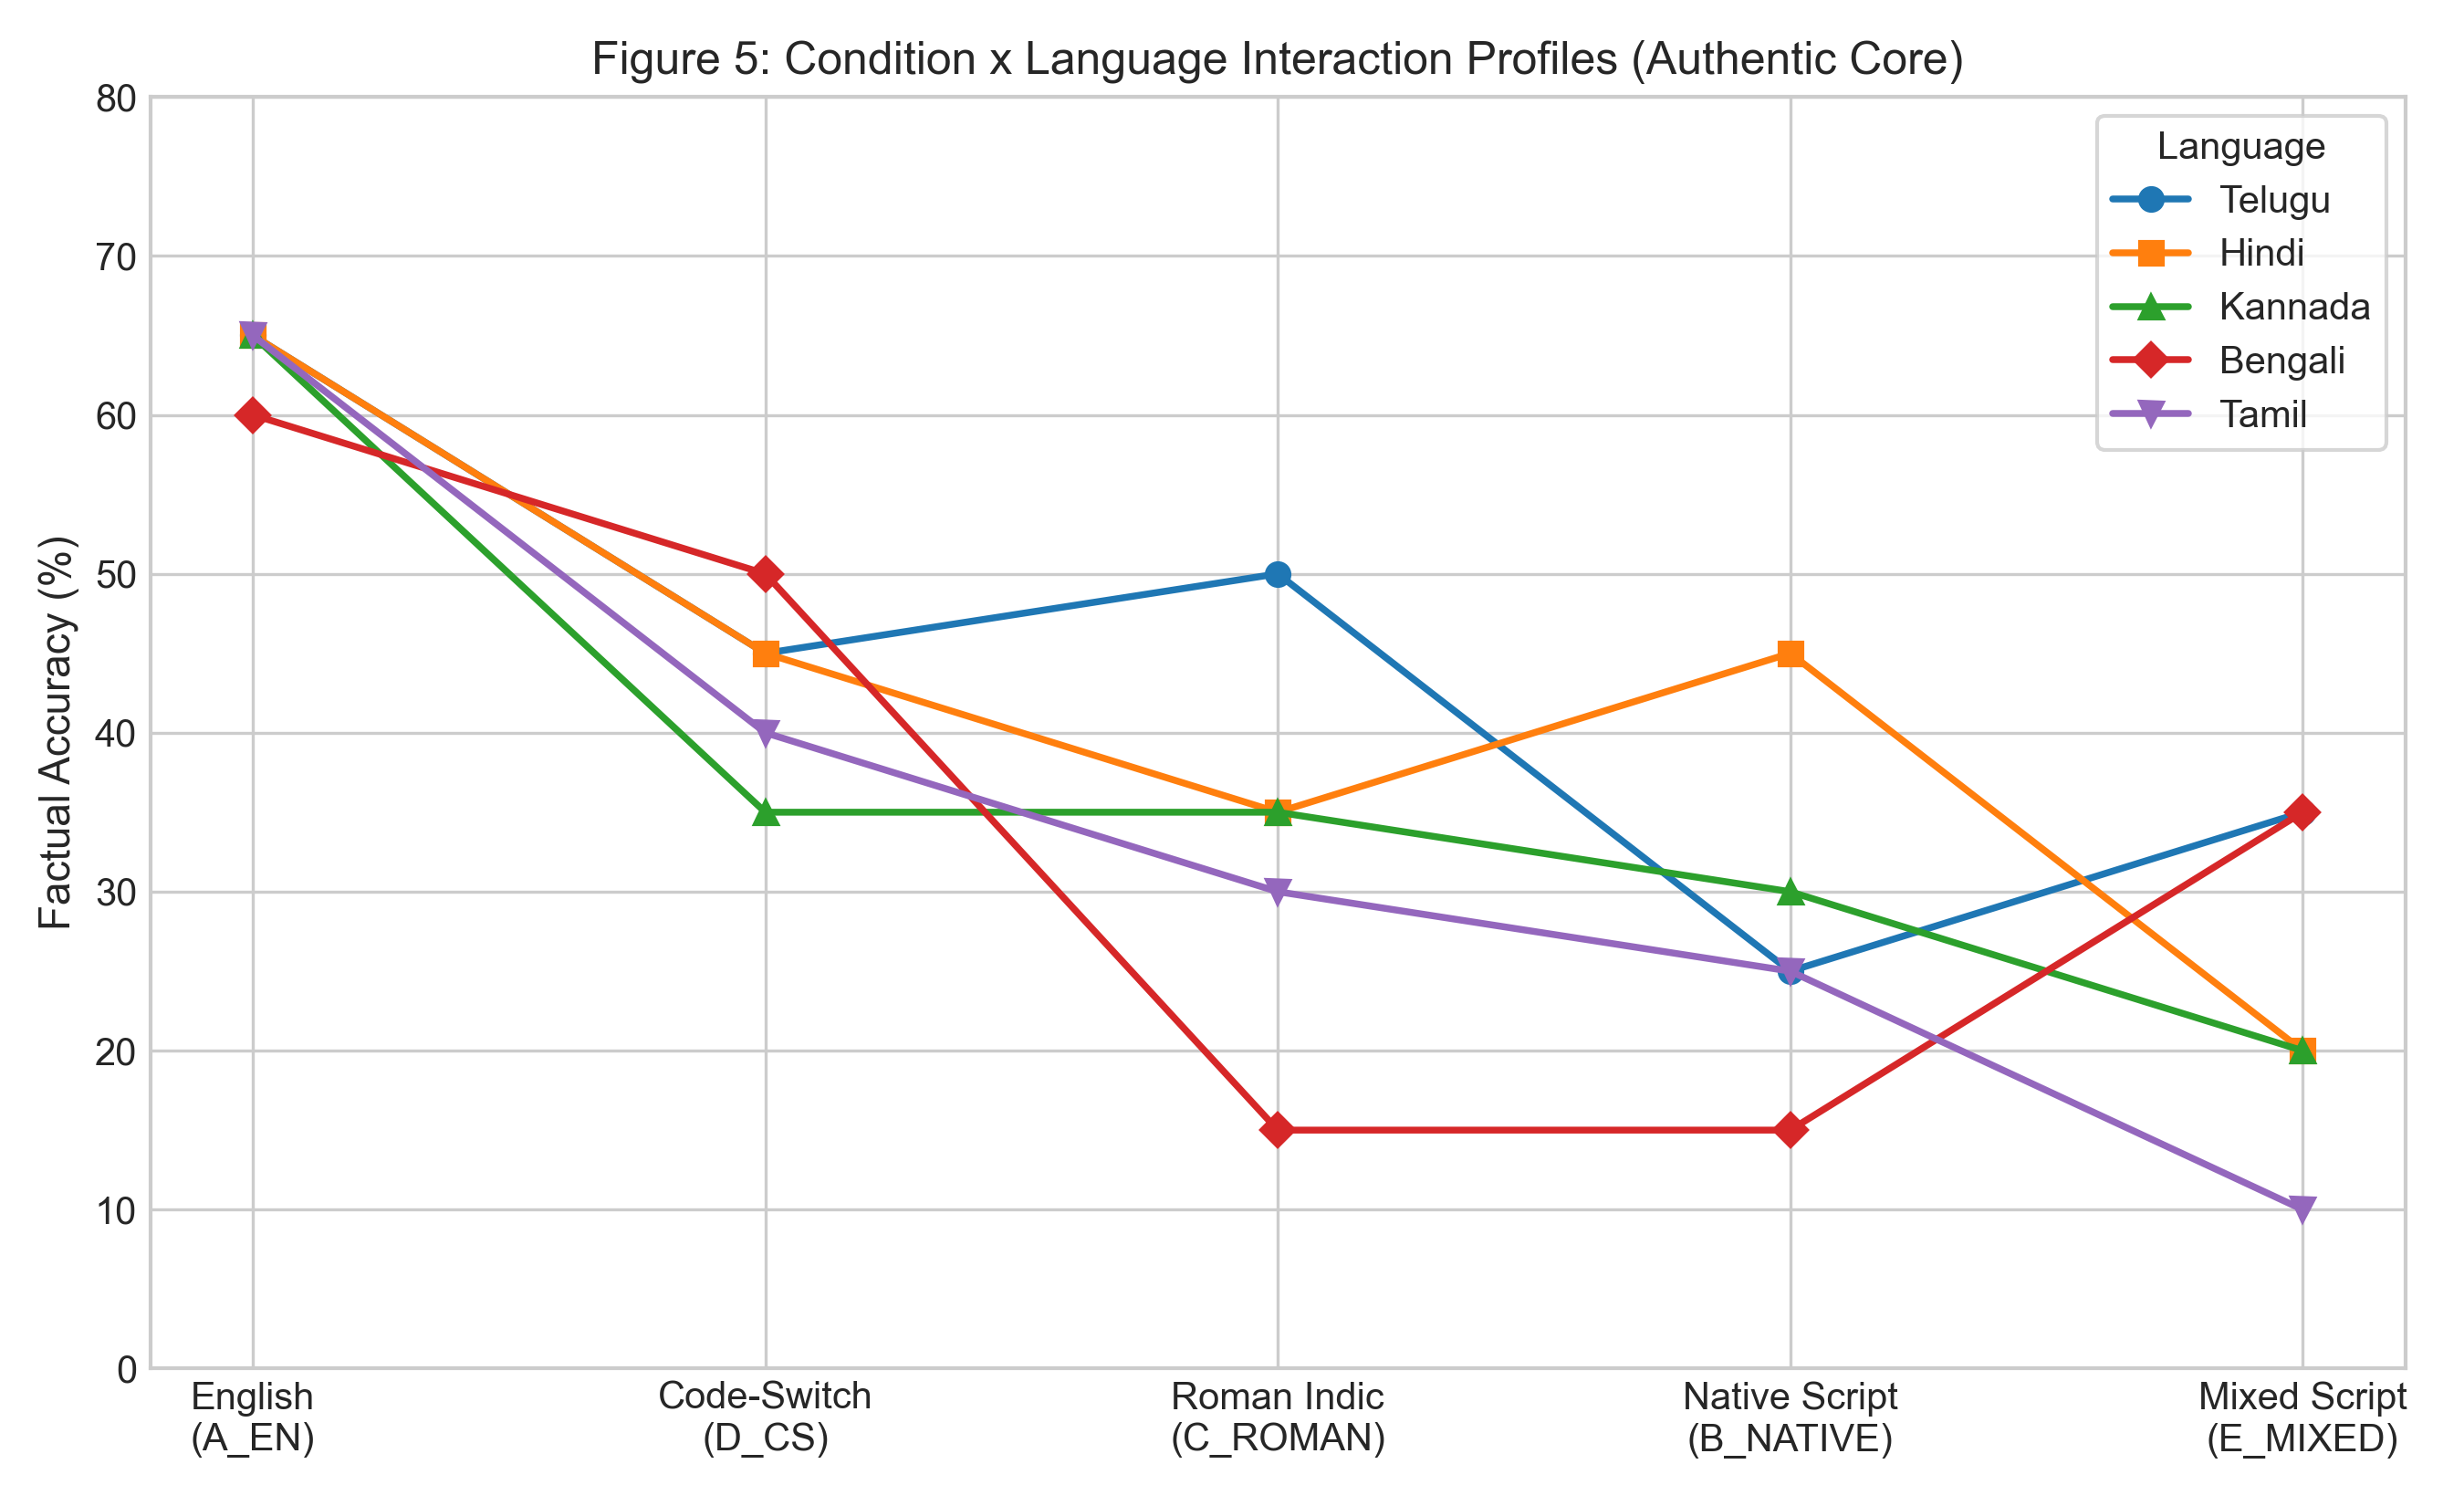
\includegraphics[width=\columnwidth]{figures/fig5_condition_x_language.png}
\caption{Condition performance profiles across five Indian languages (Authentic Policy Core, Qwen-2.5-27B).}
\label{fig:condition_x_language}
\end{figure}

\subsection{Cross-Model Comparison and Capacity Floor}
\label{sec:model_comparison}

% Table 6: Cross-Model Comparison and Capacity Floor Disclosure
\begin{table}[t]
\centering
\small
\begin{tabular}{lcccc}
\toprule
\textbf{Condition} & \textbf{Qwen-27B} & \textbf{Rank} & \textbf{Allam-7B} & \textbf{Rank} \\
\midrule
\texttt{A\_EN} & \textbf{64.0\%} & 1 & \textbf{8.0\%} & 1 \\
\texttt{D\_CS} & \textbf{43.0\%} & 2 & \textbf{5.0\%} & 2 \\
\texttt{C\_ROMAN} & \textbf{32.0\%} & 3 & \textbf{2.0\%} & 4.5 \\
\texttt{B\_NATIVE} & \textbf{28.0\%} & 4 & \textbf{2.0\%} & 4.5 \\
\texttt{E\_MIXED} & \textbf{24.0\%} & 5 & \textbf{3.0\%} & 3 \\
\midrule
\multicolumn{5}{l}{Spearman's $\rho = 0.6669$ ($p = 0.2189$, non-significant)} \\
\multicolumn{5}{l}{Kendall's $\tau = 0.5270$ ($p = 0.2326$, non-significant)} \\
\bottomrule
\end{tabular}
\caption{Cross-model performance comparison on the Authentic Policy Core ($N=100$ prompts per condition). While English and code-switching preserve their relative hierarchy across architectures, Allam-7B collapses to a capacity floor on Indic conditions (2\%--3\%), precluding fine-grained ordinal rank significance.}
\label{tab:model_comparison}
\end{table}


Table~\ref{tab:model_comparison} compares Qwen-2.5-27B against Allam-2-7B. Across both architectures, English achieves the highest accuracy and Romanized code-switching achieves the second-highest. 

However, Allam-7B collapses to a capacity floor on Indic conditions (2.0\% to 3.0\%), where inter-condition variation reflects Poisson sampling noise of a single prompt (3 vs. 2 correct completions out of 100). Consequently, while English and code-switching preserve their relative hierarchy, fine-grained cross-condition rank correlation is not statistically significant (Spearman $\rho = 0.6669, p = 0.2189$). This demonstrates that measuring subword representation dynamics requires architectures with sufficient baseline Indic pretraining capacity.

\section{Mechanistic Investigation}
\label{sec:mechanism}

% Table 8: Mechanistic Analysis of Orthographic Disruption
\begin{table*}[t]
\centering
\small
\begin{tabular}{lcccccc}
\toprule
\textbf{Condition} & \textbf{Script Transitions} & \textbf{Chars / Token} & \textbf{Accuracy} & \textbf{Reasoning Truncation} & \textbf{Numeric Drift} & \textbf{Hallucination} \\
\midrule
\texttt{A\_EN} & 0.1 & 7.12 & 64.0\% & 1.0\% & 17.0\% & 18.0\% \\
\texttt{D\_CS} & 0.1 & 6.16 & 43.0\% & 6.0\% & 33.0\% & 18.0\% \\
\texttt{C\_ROMAN} & 0.1 & 7.09 & 32.0\% & 13.0\% & 35.0\% & 20.0\% \\
\texttt{B\_NATIVE} & 1.1 & 3.26 & 28.0\% & 19.0\% & 34.0\% & 19.0\% \\
\texttt{E\_MIXED} & \textbf{5.1} & 5.23 & 24.0\% & \textbf{20.0\%} & 40.0\% & 16.0\% \\
\midrule
\multicolumn{7}{l}{\textbf{Formal Mediation Decomposition (\texttt{D\_CS} vs. \texttt{E\_MIXED}):}} \\
\multicolumn{7}{l}{Path $a$ (Condition $\to$ Chars/Token): $\beta = -0.9372$ ($p < 0.0001$); Path $c$ (Total Effect): $\beta = -0.8708$ ($p = 0.0049$)} \\
\multicolumn{7}{l}{Path $b$ (Chars/Token $\to$ Accuracy controlling for condition): $\beta = -0.0212$ ($p = 0.9387$, \textbf{Null}); Sobel $z = 0.0769$ ($p = 0.9387$, \textbf{Null})} \\
\bottomrule
\end{tabular}
\caption{Mechanistic comparison and mediation decomposition. While continuous sequence-wide token fertility does not mediate the effect (Sobel $p = 0.9387$), discrete script transitions (mean 5.1 per prompt) associate with an 18-to-20-fold surge in reasoning truncation.}
\label{tab:mechanistic_analysis}
\end{table*}


\subsection{Negative Result: Refutation of Linear Token Fertility Mediation (RQ5)}
Prior literature commonly attributes multilingual performance degradation to subword token fragmentation \citep{rust2021good,petrov2023language}. To test this hypothesis formally, we conducted a four-step Baron--Kenny mediation analysis \citep{baron1986moderator} testing whether continuous characters-per-token sequence fertility linearly mediates accuracy on the critical contrast between \texttt{D\_CS} and \texttt{E\_MIXED}.

As reported in Table~\ref{tab:mechanistic_analysis}:
\begin{itemize}
    \item \textbf{Path $a$ (Condition $\to$ Chars/Token):} Highly significant ($\beta = -0.9372, \text{SE} = 0.0792, p < 0.0001$). Dual-script prompts indeed experience severe subword fragmentation.
    \item \textbf{Path $c$ (Total Effect):} Highly significant ($\beta = -0.8708, p = 0.0049$).
    \item \textbf{Path $b$ (Chars/Token $\to$ Accuracy holding condition):} Completely null ($\beta = -0.0212, \text{SE} = 0.2762, p = 0.9387$).
    \item \textbf{Sobel Test:} Indirect effect is non-significant ($z = 0.0769, p = 0.9387$).
\end{itemize}
\textbf{Core Mechanistic Discovery:} Global sequence-wide token fertility does \textit{not} linearly mediate factual accuracy loss.

\subsection{Discrete Script Boundary Disruption}
Rather than a continuous sequence-wide dilution, error taxonomy reveals that degradation is \textit{localized and discrete}. In dual-script prompts (\texttt{E\_MIXED}), the tokenizer undergoes an average of \textbf{5.1 script transitions per prompt} (compared to 0.1 in English and code-switching).

\begin{figure}[t]
\centering
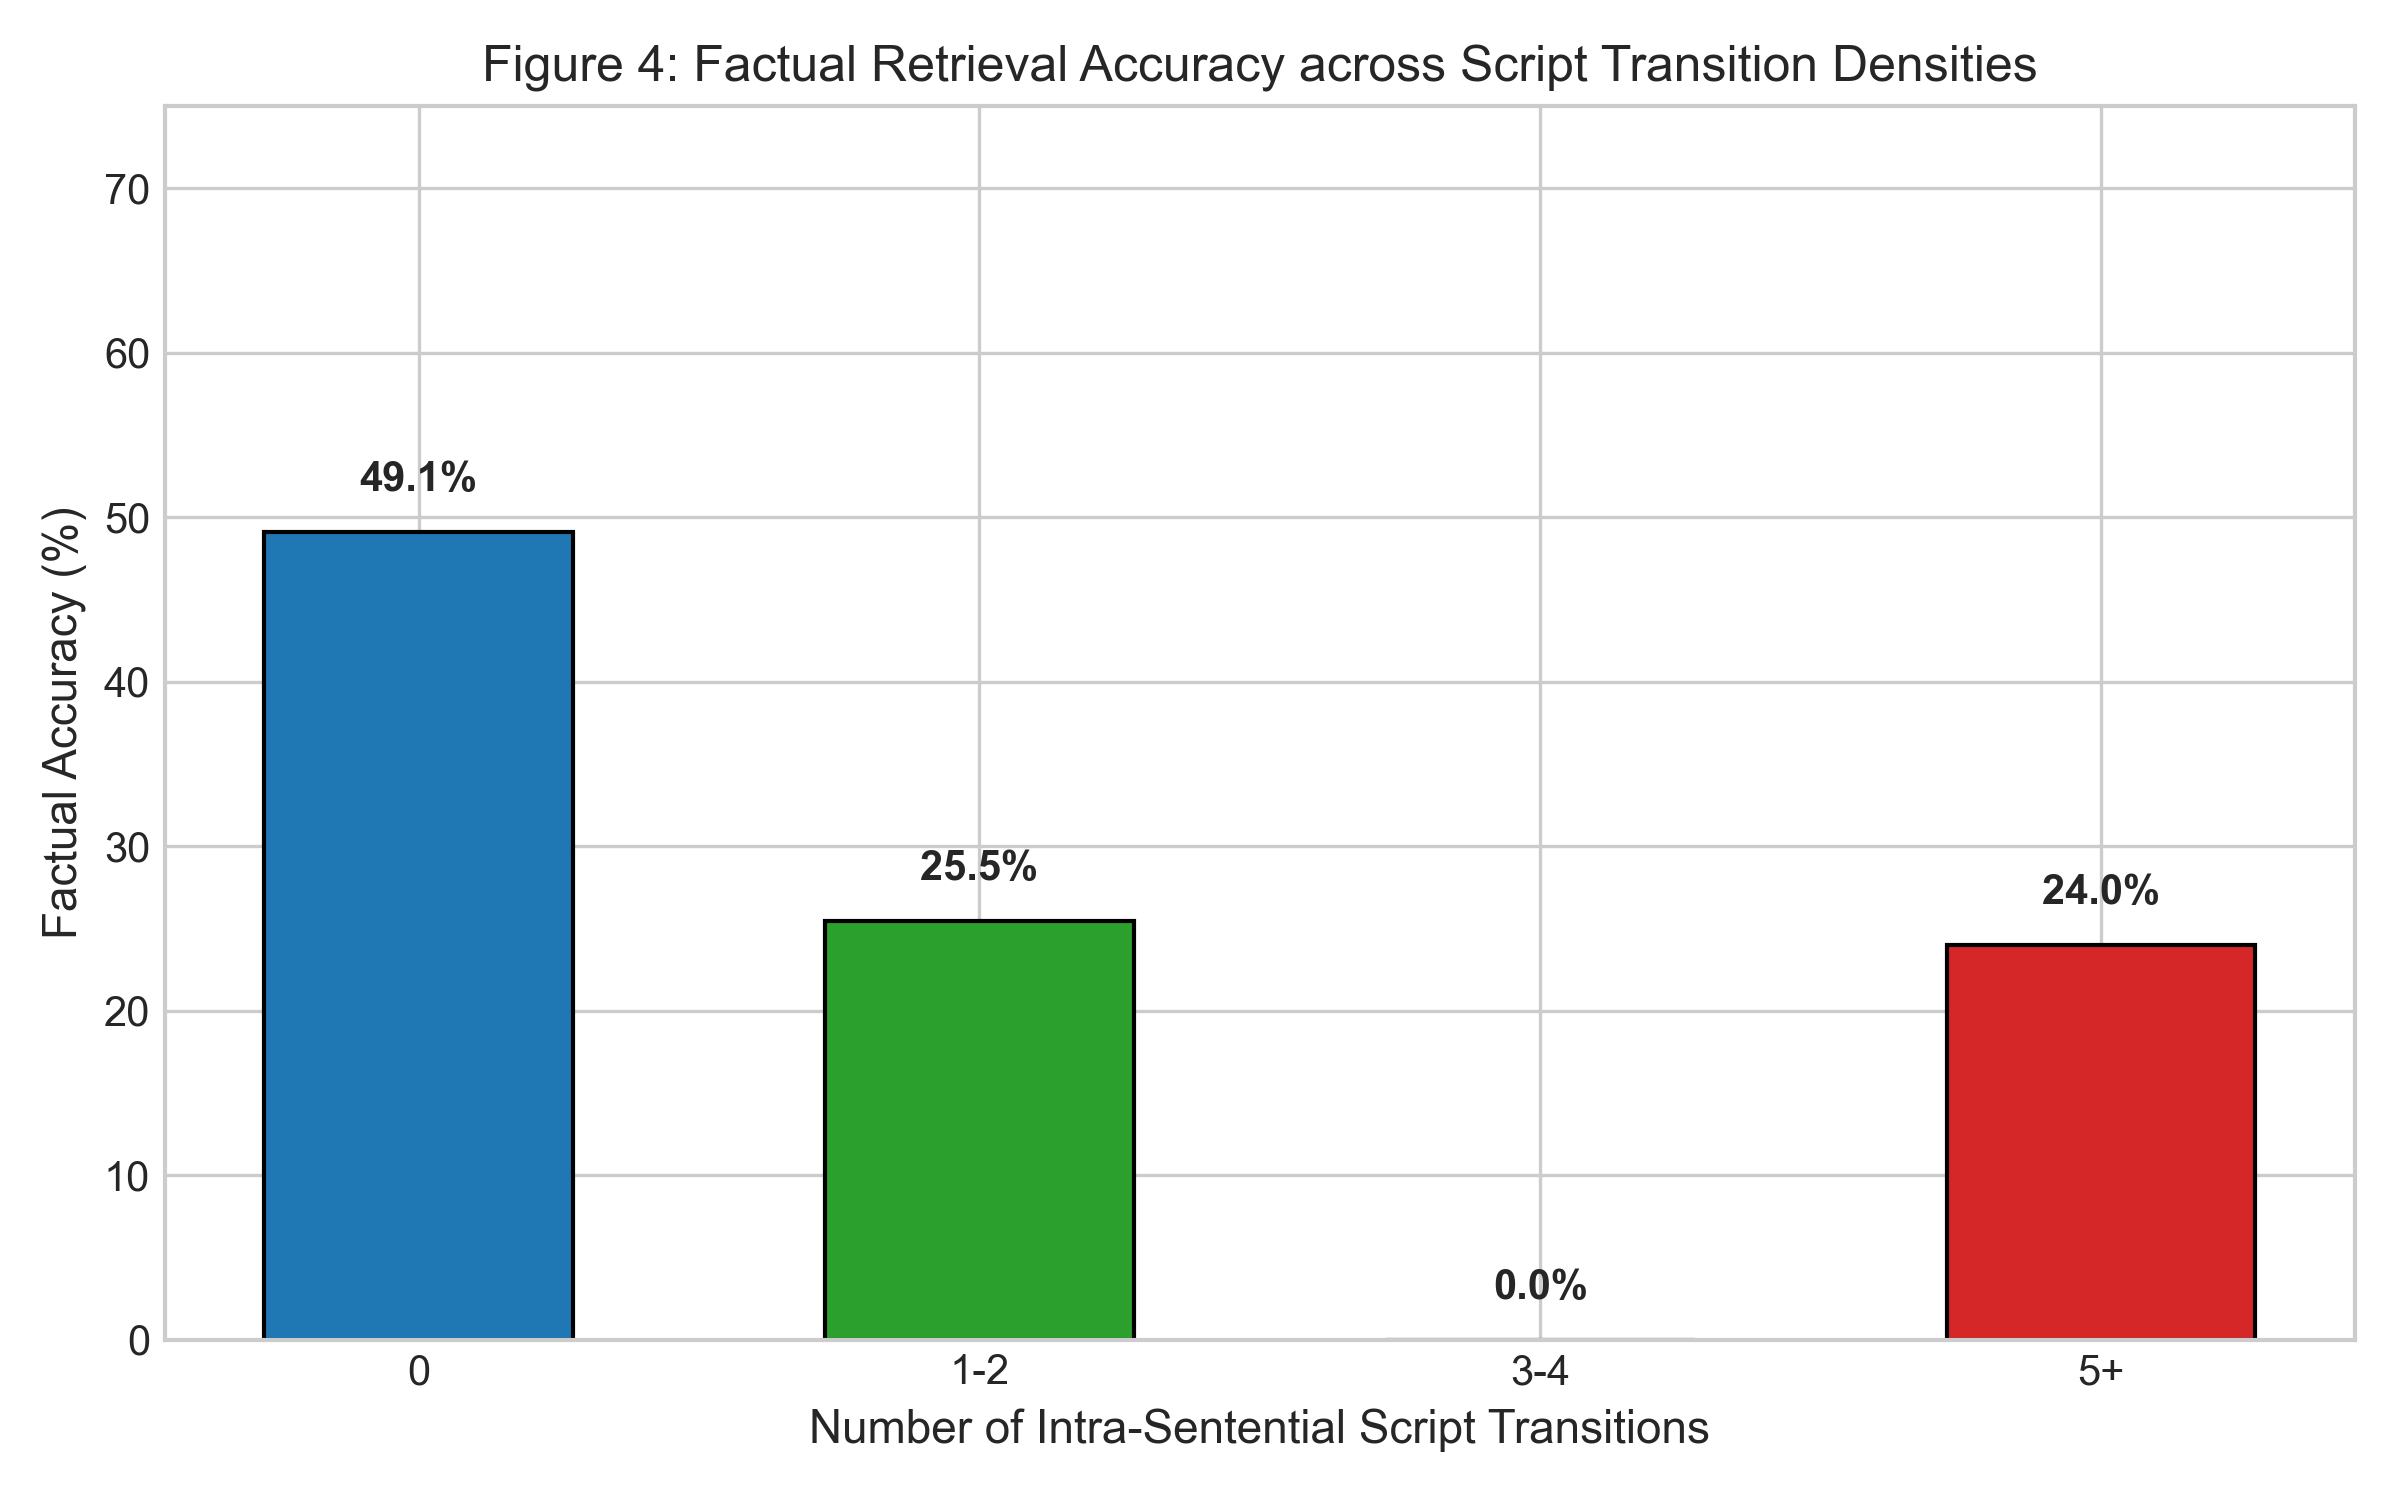
\includegraphics[width=\columnwidth]{figures/fig4_script_transitions_vs_error.png}
\caption{Factual retrieval accuracy as a function of intra-sentential script transition counts (Authentic Core).}
\label{fig:script_transitions}
\end{figure}

As shown in Figure~\ref{fig:script_transitions} and Table~\ref{tab:mechanistic_analysis}, frequent script transitions associate with a \textbf{20-fold surge in reasoning truncation} (20.0\% in \texttt{E\_MIXED} vs. 1.0\% in English). Switching writing systems mid-sentence fractures BPE subwords at boundary tokens, disrupting self-attention flow and causing generative completions to terminate prematurely before completing multi-clause statutory propositions.

\subsection{Qualitative Failure Taxonomy}
Condition-specific failure modes exhibit distinct qualitative signatures (Figure~\ref{fig:error_taxonomy}):
\begin{enumerate}
    \item \textbf{Numeric Threshold Drift (\texttt{D\_CS}):} In Romanized code-switching, errors are dominated by loss of metric precision (33.0\% vs. 17.0\% in English). Syntactic fluency and statutory domain awareness remain intact, but numbers and dates drift to adjacent salient years.
    \item \textbf{Reasoning Truncation (\texttt{E\_MIXED}):} In dual-script alternation, the model initiates correct statutory explanations but truncates before stating qualifying clauses (20.0\%).
    \item \textbf{Balanced Retrieval Omission (\texttt{A\_EN}):} In English, truncation is virtually non-existent (1.0\%), and errors reflect standard retrieval omission.
\end{enumerate}

\begin{figure}[t]
\centering
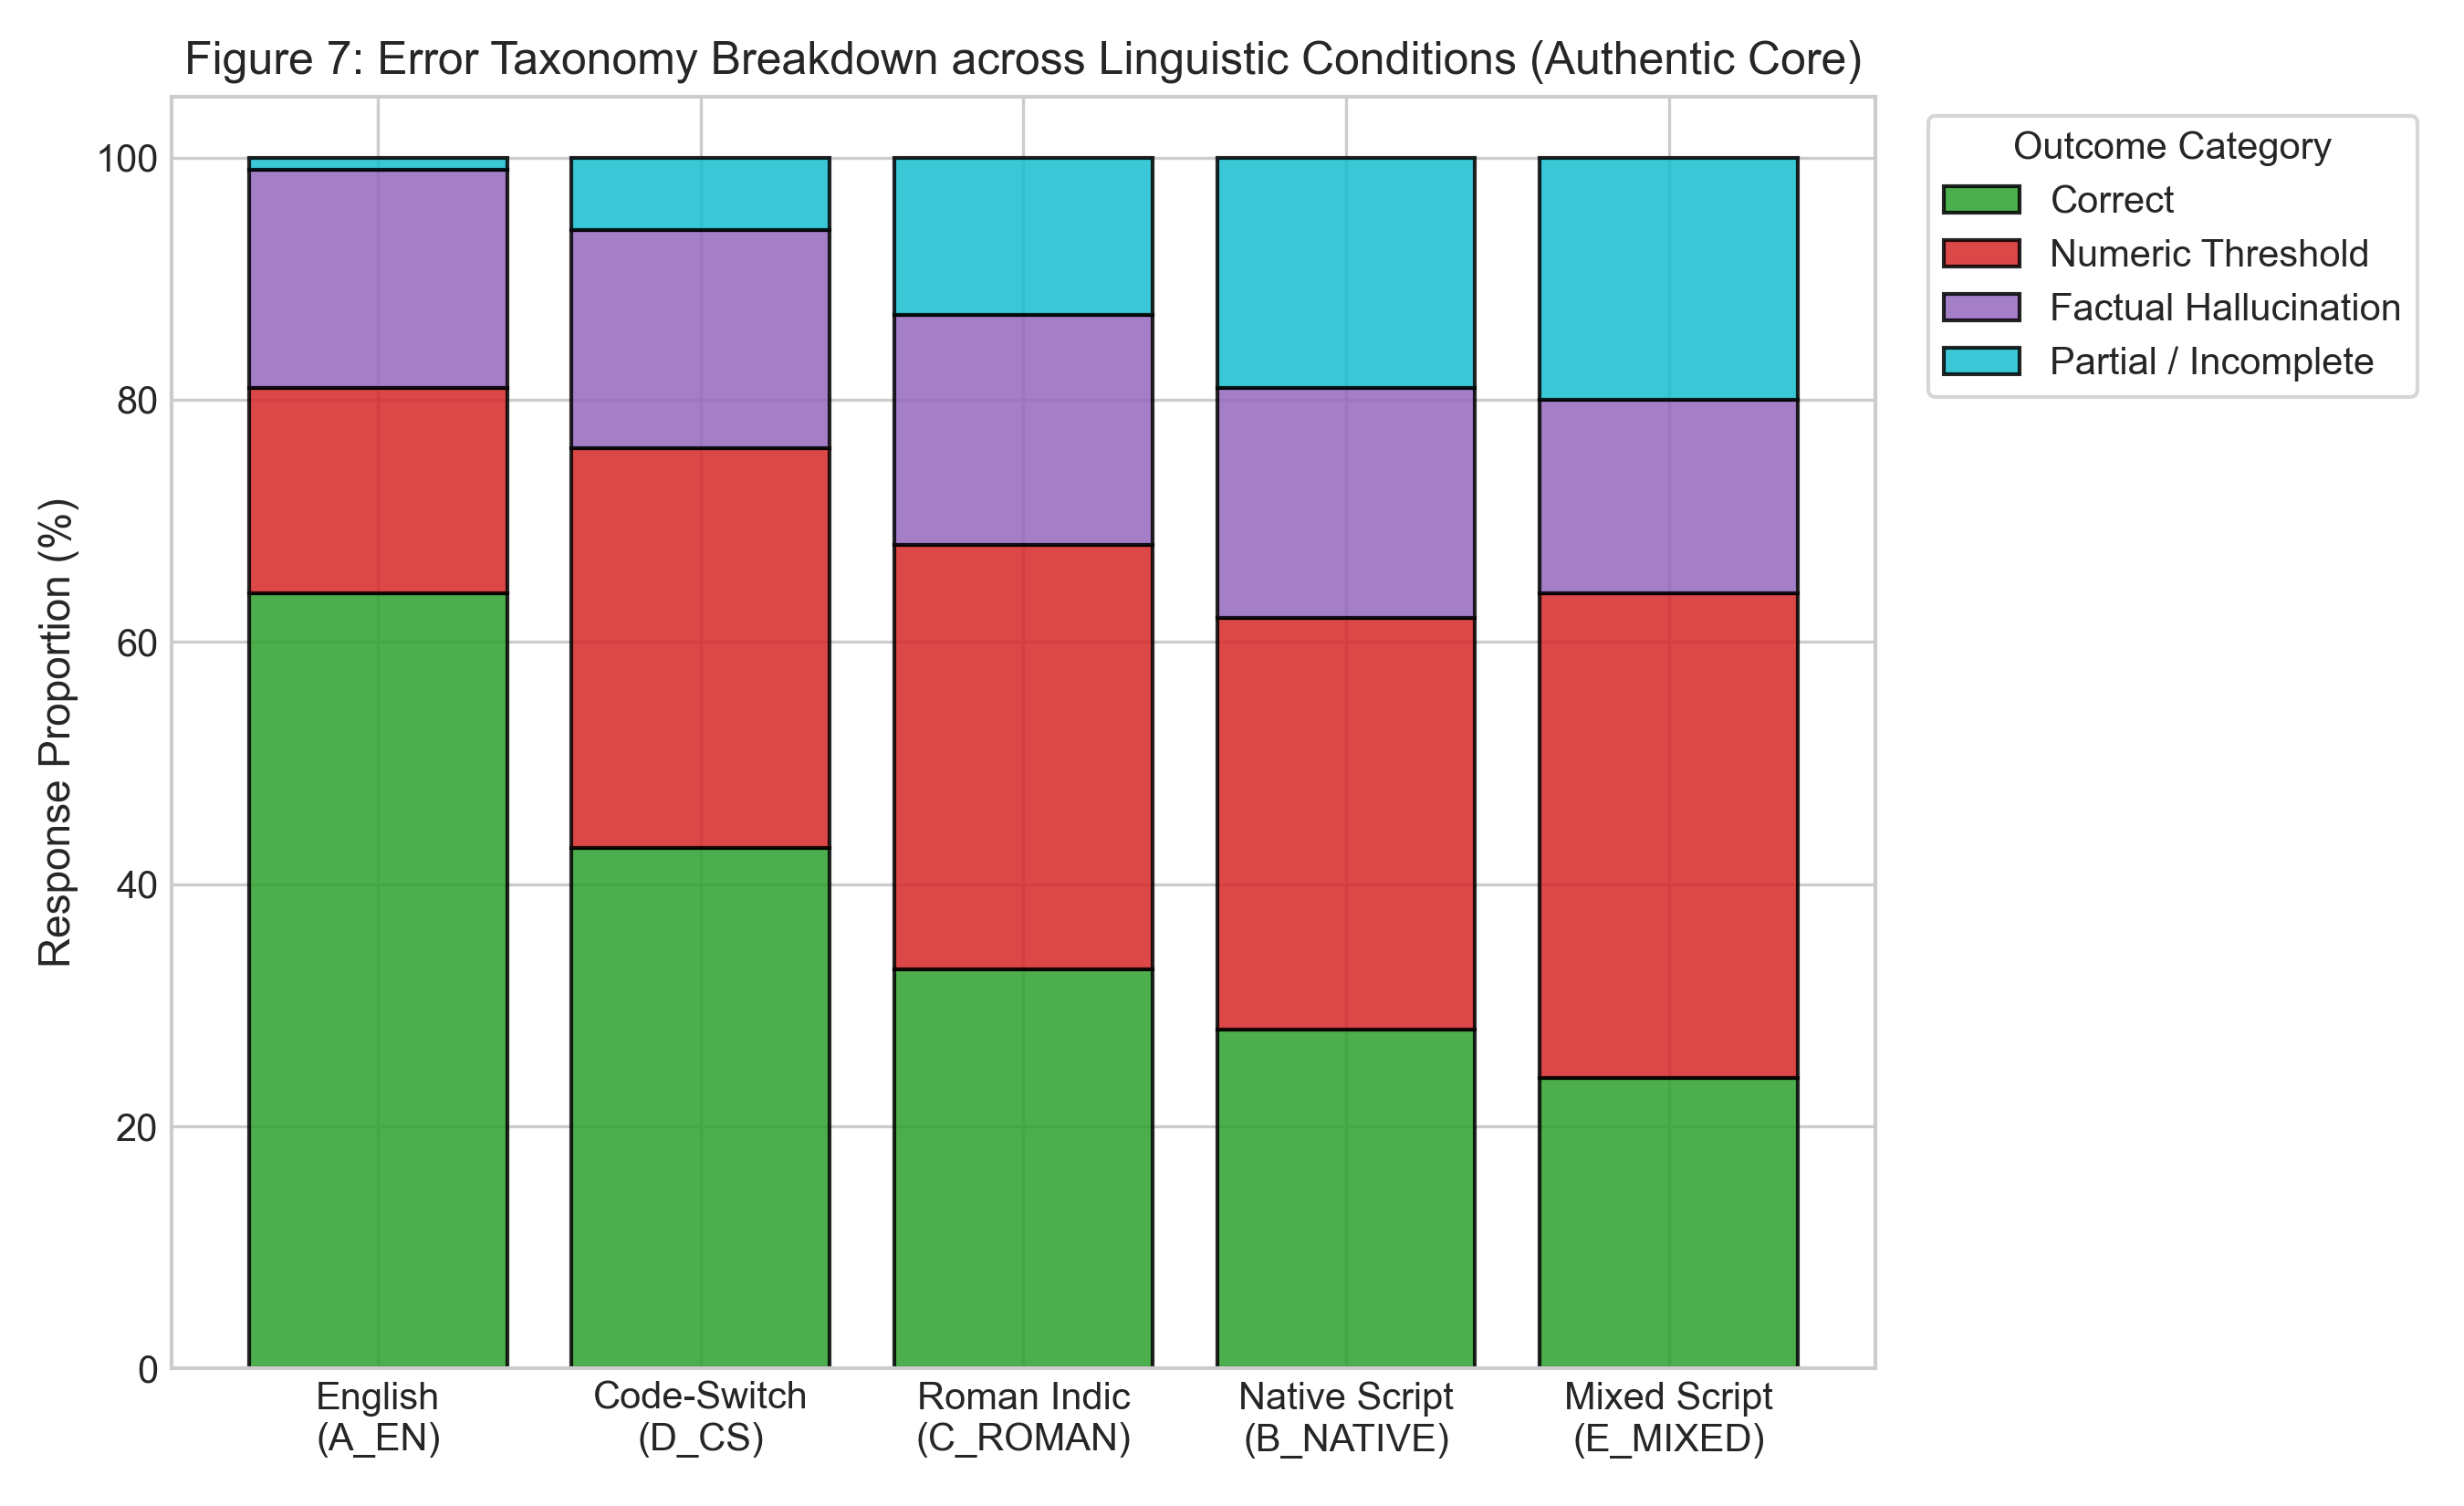
\includegraphics[width=\columnwidth]{figures/fig7_error_taxonomy_by_condition.png}
\caption{Condition-specific error taxonomy on the Authentic Policy Core ($N=100$ prompts per condition).}
\label{fig:error_taxonomy}
\end{figure}

\section{Robustness and Evaluator Sensitivity}
\label{sec:robustness}

% Table 7: Rogan--Gladen Inversion Sensitivity Grid (Selected Points)
\begin{table}[t]
\centering
\small
\begin{tabular}{ccccc}
\toprule
\textbf{CS Evaluator TPR} & \textbf{CS Evaluator FPR} & \textbf{Adj. \texttt{A\_EN}} & \textbf{Adj. \texttt{D\_CS}} & \textbf{Net Gap ($\Delta$)} \\
\midrule
0.80 & 0.04 & 68.13\% & 51.32\% & \textbf{+16.82\%} (Min) \\
0.80 & 0.10 & 68.13\% & 47.14\% & +20.99\% \\
0.84 & 0.10 & 68.13\% & 44.59\% & +23.54\% \\
\textbf{0.88} & \textbf{0.10} & \textbf{68.13\%} & \textbf{42.31\%} & \textbf{+25.82\%} (Base) \\
0.92 & 0.10 & 68.13\% & 40.24\% & +27.89\% \\
0.96 & 0.16 & 68.13\% & 33.75\% & \textbf{+34.38\%} (Max) \\
\bottomrule
\end{tabular}
\caption{Selected configurations from the 25-point 2D Rogan--Gladen sensitivity surface ($\text{TPR} \in [0.80, 0.96], \text{FPR} \in [0.04, 0.16]$). The adjusted English vs. code-switching gap remains substantial ($\ge 16.82\%$) across all tested judge measurement parameters.}
\label{tab:evaluator_sensitivity}
\end{table}


\subsection{Rogan--Gladen Latent Inversion (RQ4)}
To test whether automated LLM judge bias could artificially inflate the observed representation deficit, we applied the classical epidemiological inversion estimator of \citet{rogan1978estimating}, sweeping judge sensitivity ($\text{TPR} \in [0.80, 0.96]$) and false alarm rates ($\text{FPR} \in [0.04, 0.16]$).

As detailed in Table~\ref{tab:evaluator_sensitivity}, across all 25 parameter configurations:
\begin{itemize}
    \item \textbf{Worst-Case Leniency:} Setting $\text{TPR}=0.80, \text{FPR}=0.04$ yields adjusted English accuracy of 68.13\% and code-switching accuracy of 51.32\%, preserving a \textbf{+16.82 percentage point gap}.
    \item \textbf{Base Point Estimate:} Using human-validated error rates ($\text{TPR}=0.88, \text{FPR}=0.10, \kappa = 0.824$) yields an adjusted gap of \textbf{+25.82 percentage points}.
\end{itemize}
The performance gap never closes or reverses, confirming that evaluator measurement error alone cannot account for the representation deficit.

\section{Prospective Benchmark Expansion}
\label{sec:expansion}

To resolve the sample size constraint of the 20-topic baseline, we constructed and released \textbf{IndraLLM-CS-v1.2-PILOT}:
\begin{itemize}
    \item \textbf{Scale:} 25 brand-new, independent statutory acts (\texttt{AUTH-021} to \texttt{AUTH-045}), yielding 125 multi-condition prompts.
    \item \textbf{Independence Verification:} Automated audits verified zero entity collisions ($0/25$) and negligible evidence n-gram overlap ($J \le 0.0208$) against the original core.
    \item \textbf{Prospective Power:} Expanding the benchmark design from 20 to 45 topics elevates the prospective effective sample size to $N_{\text{eff}} = 152.2$ and prospective statistical power to \textbf{88.6\% (exact: 88.57\%)} ($\text{MDE} = 18.60\%$).
\end{itemize}
We emphasize that this 45-topic expansion represents a frozen benchmark release and prospective power calculation; empirical inference in this paper covers the 20-topic authentic core.

\section{Limitations}
\label{sec:limitations}

We explicitly delineate the boundary conditions of this study:
\begin{enumerate}
    \item \textbf{Topic-Level Sample Size:} The empirical core comprises 20 statutory frameworks ($N=500$ prompts). While native Indic and dual-script drops remain $p \le 0.0005$, the code-switching contrast yields $p = 0.0528$ at the statutory act cluster level due to cluster dependence ($55.9\%$ power).
    \item \textbf{Prospective Expansion Status:} The 25 pilot topics have been constructed, audited, and released, but have not yet undergone live model inference.
    \item \textbf{Model Scope:} Evaluations were conducted on two open-weight architectures (Qwen-2.5-27B and Allam-2-7B). Results do not extrapolate to all LLM architectures universally.
    \item \textbf{Capacity Floor in Smaller Models:} Allam-7B exhibits a 2\%--3\% capacity floor on Indic conditions, precluding fine-grained ordinal ranking.
    \item \textbf{Parametric vs. RAG Retrieval:} Our study measures closed-book parametric recall. We make no claims regarding whether retrieval-augmented generation (RAG) with in-context gold snippets mitigates the penalty.
    \item \textbf{Language Scope:} Evaluations cover five major scheduled languages. We make no claims regarding unrepresented language families or unwritten vernaculars.
    \item \textbf{Associational Mechanism:} The link between script transition density and reasoning truncation is an empirical association, not a mathematically demonstrated causal neural proof.
\end{enumerate}

\section{Ethics and Responsible Use}
\label{sec:ethics}

Our findings analyze model vulnerabilities under non-canonical linguistic encodings. We explicitly emphasize that observed accuracy deficits reflect \textbf{systemic limitations in LLM pretraining corpora and subword tokenizers}, not inherent deficiencies in the Indian languages or code-switching varieties themselves. Code-switching is a natural, highly structured, and cognitively rich sociolinguistic phenomenon. Systems deployed in multilingual public administration must be engineered to treat non-canonical inputs with the same factual precision as standard English.

\section{Conclusion}
\label{sec:conclusion}

Through strict five-way semantic pairing on authentic Indian statutory law, IndraLLM demonstrates that Large Language Model factual recall is fragile to surface linguistic representation. Models capable of answering factual questions in English suffer severe degradation under code-switched and mixed-script representations. We refute the hypothesis that global sequence token fertility linearly mediates this loss, identifying discrete orthographic transition boundaries as the primary driver of reasoning truncation. By disclosing topic-level clustering limitations and releasing an expanded 45-topic benchmark architecture, this work provides a rigorous foundation for evaluating and hardening multilingual knowledge systems.

\bibliographystyle{plain}
\bibliography{references}

\clearpage
\appendix
\section{Annotation Guidelines and Quality Control}
\label{sec:supp_annotation}

To ensure high ecological validity and linguistic naturalness while strictly maintaining factual invariance, all prompts in IndraLLM were constructed following standardized annotation procedures:

\begin{enumerate}
    \item \textbf{Semantic Invariance Principle:} Every condition realization (\texttt{A\_EN}, \texttt{B\_NATIVE}, \texttt{C\_ROMAN}, \texttt{D\_CS}, \texttt{E\_MIXED}) must query the exact same statutory entity, parameter, date, or threshold. No condition may introduce extraneous legal hints or omit required qualifying constraints.
    \item \textbf{Code-Switching Conventions (\texttt{D\_CS}):} Romanized code-switching mirrors informal conversational communication across urban Indian digital contexts (e.g., Hinglish, Tanglish, Tenglish). Function words and conversational framing are provided in the Indic language using standardized Latin transliteration, while technical statutory nouns and act titles (e.g., \textit{Consumer Protection Act}, \textit{pecuniary jurisdiction}, \textit{threshold}) remain in English.
    \item \textbf{Dual-Script Conventions (\texttt{E\_MIXED}):} Intra-sentential script alternation inserts technical English acronyms and nouns in Latin script directly into native Brahmic script sentences (Devanagari, Tamil, Telugu, Bengali, Kannada), reflecting common web and administrative document layouts.
    \item \textbf{Inter-Annotator Agreement:} Native speaker validation across five Indian languages yielded a Fleiss' $\kappa = 0.719$ and Krippendorff's $\alpha = 0.719$, confirming substantial agreement on semantic equivalence and naturalness (mean naturalness score: $4.74 / 5.0$).
\end{enumerate}

\section{Prompt Templates and 5-Way Realization Examples}
\label{sec:supp_prompts}

Table~\ref{tab:supp_prompt_examples} provides verbatim examples across all five evaluated Indian languages for Topic \texttt{AUTH-006} (Citizenship Amendment Act Cut-off Date).

\begin{table*}[t]
\centering
\small
\begin{tabular}{llp{11.5cm}}
\toprule
\textbf{Language} & \textbf{Condition} & \textbf{Verbatim Query Text} \\
\midrule
All & \texttt{A\_EN} & Under the Citizenship Amendment Act 2019, what is the prerequisite statutory cut-off date for eligible migrants? \\
\midrule
Hindi (\texttt{hi}) & \texttt{B\_NATIVE} & नागरिकता संशोधन अधिनियम 2019 के अनुसार, पात्र प्रवासियों के लिए वैधानिक कट-ऑफ तिथि क्या है? \\
Hindi (\texttt{hi}) & \texttt{C\_ROMAN} & Nagrikta sanshodhan adhiniyam 2019 ke anusar, patra pravasiyon ke liye vaaidhanik cut-off tareekh kya hai? \\
Hindi (\texttt{hi}) & \texttt{D\_CS} & CAA cut-off date ke hisaab se eligible migrants ke liye statutory prerequisite timeline kya hai? \\
Hindi (\texttt{hi}) & \texttt{E\_MIXED} & CAA cut-off date के हिसाब से eligible migrants के लिए statutory prerequisite timeline क्या है? \\
\midrule
Tamil (\texttt{ta}) & \texttt{B\_NATIVE} & குடியுரிமை திருத்தச் சட்டம் 2019 இன் படி, தகுதியான குடியேறியவர்களுக்கான சட்டப்பூர்வ காலக்கெடு தேதி என்ன? \\
Tamil (\texttt{ta}) & \texttt{C\_ROMAN} & Kudiyurimai thiruthach sattam 2019 in padi, thagudhiyaana kudiyeriyavargalukkaana sattappoorva kaalakkedu thedhi enna? \\
Tamil (\texttt{ta}) & \texttt{D\_CS} & CAA cut-off date prakaram eligible migrants-kku statutory prerequisite timeline enna? \\
Tamil (\texttt{ta}) & \texttt{E\_MIXED} & CAA cut-off date ప్రకారం eligible migrants-க்கு statutory prerequisite timeline என்ன? \\
\midrule
Telugu (\texttt{te}) & \texttt{B\_NATIVE} & పౌరసత్వ సవరణ చట్టం 2019 ప్రకారం, అర్హులైన వలసదారులకు చట్టబద్ధమైన గడువు తేదీ ఏమిటి? \\
Telugu (\texttt{te}) & \texttt{C\_ROMAN} & Pourasathva savarana chattam 2019 prakaram, arhulaiana valasadhaarulaku chattabaddhamaina gaduvu thedhee emiti? \\
Telugu (\texttt{te}) & \texttt{D\_CS} & CAA cut-off date prakaram eligible migrants kosam statutory prerequisite timeline enti? \\
Telugu (\texttt{te}) & \texttt{E\_MIXED} & CAA cut-off date ప్రకారం eligible migrants కోసం statutory prerequisite timeline ఏమిటి? \\
\bottomrule
\end{tabular}
\caption{Representative 5-way semantic-paired prompts querying Topic \texttt{AUTH-006} (CAA Cut-off Date: December 31, 2014) across Hindi, Tamil, and Telugu.}
\label{tab:supp_prompt_examples}
\end{table*}

\section{Mathematical and Statistical Derivations}
\label{sec:supp_statistics}

\subsection{Intra-Cluster Correlation and Clustered Design Effect}
In cluster-correlated evaluation where observations are clustered within legislative acts $j \in \{1, \dots, K\}$, total variance decomposes into between-cluster variance $\sigma^2_{\text{topic}}$ and residual within-cluster variance $\sigma^2_{\text{residual}}$:
\begin{equation}
\text{ICC} = \rho = \frac{\sigma^2_{\text{topic}}}{\sigma^2_{\text{topic}} + \sigma^2_{\text{residual}}}
\end{equation}
Empirically estimated via a linear mixed-effects model on the Authentic Policy Core ($N=500$ prompts across 20 acts):
\begin{equation}
\sigma^2_{\text{topic}} = 0.0588, \quad \sigma^2_{\text{residual}} = 0.1619 \implies \text{ICC} = 0.2663
\end{equation}

For cluster size $m$, the survey Design Effect ($\text{DEFF}$) measures variance inflation relative to simple random sampling:
\begin{equation}
\text{DEFF} = 1 + (m - 1)\rho
\end{equation}
For overall dataset evaluation ($m = 25$ prompts per statutory topic):
\begin{equation}
\text{DEFF}_{\text{full}} = 1 + (25 - 1)(0.2663) = 7.3912 \implies N_{\text{eff}} = \frac{500}{7.3912} = 67.64
\end{equation}

For pairwise condition contrasts (e.g., \texttt{A\_EN} vs. \texttt{D\_CS}), each cluster contains $m_{\text{cond}} = 5$ prompts:
\begin{equation}
\text{DEFF}_{\text{cond}} = 1 + (5 - 1)(0.2663) = 2.0652
\end{equation}
The standard error of the proportion difference $\Delta = p_1 - p_2$ across $K$ clusters is:
\begin{equation}
\text{SE}_{\Delta} = \sqrt{\frac{2 \cdot \bar{p}(1 - \bar{p}) \cdot \text{DEFF}_{\text{cond}}}{K \cdot m_{\text{cond}}}}
\end{equation}
For $K = 20$ topics: $\text{SE}_{\Delta} = 0.0996$, yielding statistical power for $\Delta = 0.21$:
\begin{equation}
z = \frac{0.21 - 1.96(0.0996)}{0.0996} = 0.14925 \implies \Phi(z) = 55.93\%
\end{equation}
For $K = 45$ expanded topics: $\text{SE}_{\Delta} = 0.0664$, yielding prospective power:
\begin{equation}
z = \frac{0.21 - 1.96(0.0664)}{0.0664} = 1.2038 \implies \Phi(z) = 88.57\% \approx 88.6\%
\end{equation}

\subsection{Rogan--Gladen Latent Inversion Estimator}
Let $P_{\text{obs}}$ denote the apparent accuracy assigned by an automated judge with sensitivity $\text{TPR} = P(\hat{Y}=1 \mid Y=1)$ and false-positive rate $\text{FPR} = P(\hat{Y}=1 \mid Y=0)$. By total probability:
\begin{equation}
P_{\text{obs}} = \pi \cdot \text{TPR} + (1 - \pi) \cdot \text{FPR}
\end{equation}
Solving for the true latent accuracy $\pi$:
\begin{equation}
\pi = \frac{P_{\text{obs}} - \text{FPR}}{\text{TPR} - \text{FPR}}
\end{equation}
To ensure validity on the probability simplex, estimates are bounded: $\hat{\pi} = \max(0.0, \min(1.0, \pi))$.

\section{Dataset Architecture and Error Taxonomy}
\label{sec:supp_dataset_taxonomy}

\subsection{Benchmark Partitions and Contamination Controls}
IndraLLM enforces strict isolation between evaluation partitions:
\begin{itemize}
    \item \textbf{Development Partition (5,000 prompts, 1,000 groups):} Assigned exclusively to Template Families \texttt{TF-01} through \texttt{TF-06}.
    \item \textbf{Validation Partition (1,000 prompts, 200 groups):} Assigned to Template Families \texttt{TF-07} and \texttt{TF-08}.
    \item \textbf{Test-ID Partition (1,000 prompts, 200 groups):} In-distribution testing using disjoint entities under \texttt{TF-09} and \texttt{TF-10}.
    \item \textbf{Test-OOD Partition (500 prompts, 100 groups):} Out-of-distribution evaluation under novel structural syntactic frames (\texttt{TF-11}, \texttt{TF-12}).
    \item \textbf{Authentic Statutory Core (500 prompts, 100 groups):} Embedded within the test partition; comprises 20 legally enacted Indian statutory acts derived from official Ministry gazettes.
\end{itemize}

\subsection{Qualitative Failure Taxonomy Definitions}
Incorrect model completions were classified into four discrete failure modes:
\begin{enumerate}
    \item \textbf{Numeric Threshold Drift:} The model retrieves the correct statute, legal context, and qualitative condition, but misreports a numerical threshold, penalty limit, or year (e.g., retrieving December 31, 2019 instead of December 31, 2014 for the CAA cut-off date). Dominant in Romanized code-switching (\texttt{D\_CS}, 33.0\%).
    \item \textbf{Reasoning Truncation and Incompleteness:} The completion initiates a relevant explanation but terminates prematurely mid-sentence or mid-clause, omitting the defining comparative or relational counterpart. Dominant in dual-script alternation (\texttt{E\_MIXED}, 20.0\% vs. 1.0\% in English).
    \item \textbf{Factual Hallucination / Distortion:} The model invents non-existent provisions, attributes rules to unrelated governmental bodies (e.g., fabricating National Informatics Centre departments), or confounds distinct statutes.
    \item \textbf{Refusal / Evasion:} The model issues a standard refusal string (e.g., claiming inability to answer or demanding additional context).
\end{enumerate}

\subsection{Preserved Negative Results}
In accordance with open science practices, we document two major null findings:
\begin{enumerate}
    \item \textbf{Global Token Fertility Mediation Null:} Baron--Kenny Path $b$ testing whether continuous characters-per-token sequence fertility linearly mediates accuracy was non-significant ($\beta = -0.0212, p = 0.9387$, Sobel $z = 0.0769$). Sequence-wide token counts do not drive the factual deficit.
    \item \textbf{Cross-Model Rank Invariance Null:} On the Authentic Core, Allam-7B collapses to a capacity floor on Indic conditions (2\%--3\%), resulting in a non-significant Spearman correlation ($\rho = 0.6669, p = 0.2189$). Measuring representation sensitivity requires models with sufficient baseline Indic pretraining capacity.
\end{enumerate}


\end{document}
